%% MSc Thesis — main.tex
%% IDEA League visual design + working_template file structure
%% Compiler: LuaLaTeX → biber → LuaLaTeX × 2
%%
\documentclass[a4paper,11pt,twoside,openright]{report}
%
% ── Thesis metadata ──────────────────────────────────────────────────────────
\newcommand{\mythesistitle}{From Particles to Waves}
\newcommand{\mysubtitle}{Towards coupling Dynamic Snow Modelling and Spectral Elements to detect Avalanche Breakoff in DAS Data.}
\newcommand{\myauthor}{Salome Anna Bachmann}
\newcommand{\mysupervisor}{Johannes Aichele \textbar{} Pascal Edme \textbar{} Johan Gaume}
\newcommand{\myreaderone}{Johannes Aichele}
\newcommand{\myreadertwo}{Pascal Edme}
\newcommand{\myreaderthree}{Johan Gaume}   % leave blank {} if unused
\newcommand{\myinstitution}{IDEA LEAGUE \textbar{} ETH Zürich}
\newcommand{\mydate}{\today}
%
% ── Preamble (packages, colours, commands) ───────────────────────────────────
% tex/preamble.tex
% ──────────────────────────────────────────────────────────────────────────────
% Packages
% ──────────────────────────────────────────────────────────────────────────────
\usepackage[a4paper, margin=2.5cm, bindingoffset=0.5cm]{geometry}
\usepackage[english]{babel}
\usepackage{fancyhdr}
\usepackage{csquotes}
\usepackage{emptypage}            % suppresses headers on blank pages

% ── Fonts ─────────────────────────────────────────────────────────────────────
\usepackage{isomath}
\usepackage{mathtools}
\usepackage{amsthm}
\usepackage[scaled=0.98,sups]{XCharter}
\usepackage[scaled=0.94,ttdefault,type1]{sourcecodepro}
\usepackage[type1]{sourcesanspro}
\usepackage[xcharter,vvarbb,scaled=1.13]{newtxmath}

% ── Figures & tables ──────────────────────────────────────────────────────────
\usepackage{graphicx}
\usepackage[font=sf,bf,justification=centering]{caption}
\captionsetup[table]{position=top}
\usepackage[font=sf]{floatrow}
\usepackage{subcaption}
\usepackage{booktabs}
\usepackage{wrapfig}

% ── Layout & spacing ──────────────────────────────────────────────────────────
\usepackage{parskip}
\usepackage[titles]{tocloft}
\usepackage{multicol}
\usepackage{enumitem}
\usepackage{anyfontsize}

% ── Science & units ───────────────────────────────────────────────────────────
\usepackage[exponent-product=\cdot]{siunitx}
\usepackage{chemmacros}

% ── Code listings ─────────────────────────────────────────────────────────────
\usepackage{listings}
\usepackage{lstautogobble}

% ── Colour ────────────────────────────────────────────────────────────────────
\usepackage{xcolor}
\usepackage[most]{tcolorbox}

% ── TikZ ──────────────────────────────────────────────────────────────────────
\usepackage{tikz}
\usetikzlibrary{shapes.geometric, arrows.meta, positioning}

% ── Date ──────────────────────────────────────────────────────────────────────
\usepackage[showdow,en-US]{datetime2}

% ── Appendix ──────────────────────────────────────────────────────────────────
\usepackage[titletoc]{appendix}

% ── IDEA League chapter heading style (fncychap "Bjarne" ruled style) ─────────
\usepackage{fncychap}
\makeatletter
  \ChNameVar{\raggedleft\Large\sffamily}
  \ChNumVar{\Large\sffamily}
  \ChTitleVar{\raggedleft\Huge\sffamily\bfseries}
  \ChRuleWidth{2pt}
  \renewcommand{\DOCH}{%
    \vskip -0.5\baselineskip
    \mghrulefill{\RW}\par\nobreak
    \CNV\FmN{\@chapapp}\space\CNoV\thechapter
    \par\nobreak
    \vskip -0.5\baselineskip
  }
  \renewcommand{\DOTI}[1]{%
    \mghrulefill{\RW}\par\nobreak
    \CTV\FmTi{#1}\par\nobreak
    \vskip 50\p@
  }
  \renewcommand{\DOTIS}[1]{%
    \mghrulefill{\RW}\par\nobreak
    \CTV\FmTi{#1}\par\nobreak
    \vskip 50\p@
  }
\makeatother

% ── Title decoration (for cover page) ─────────────────────────────────────────
\usepackage{eso-pic}              % AddToShipoutPicture
\usepackage{pdfpages}             % \includepdf

% ── Font encoding (pdflatex fallback) ─────────────────────────────────────────
\ifdefined\directlua\else
  \usepackage[T1]{fontenc}
\fi

% ──────────────────────────────────────────────────────────────────────────────
% Bibliography  (lualatex → biber → lualatex × 2)
% ──────────────────────────────────────────────────────────────────────────────
\usepackage[
  style=authoryear,
  sorting=nyt,
  maxbibnames=5,
  maxcitenames=2,
  giveninits=true,
  uniquelist=false,
  uniquename=init,
  seconds=true,
  url=false,
  backend=biber,
]{biblatex}
\addbibresource{../../master_thesis.bib}
\DeclareDelimFormat{nameyeardelim}{\addcomma\space}
\newcommand\citep{\parencite}

% ──────────────────────────────────────────────────────────────────────────────
% ETH Zürich / IDEA League colours
% ──────────────────────────────────────────────────────────────────────────────
\definecolor{eth-blau}{RGB}{33,92,175}
\definecolor{eth-petrol}{RGB}{0,120,148}
\definecolor{eth-grun}{RGB}{98,115,19}
\definecolor{eth-bronze}{RGB}{142,103,19}
\definecolor{eth-rot}{RGB}{183,53,45}
\definecolor{eth-purpur}{RGB}{167,17,122}
\definecolor{eth-grau}{RGB}{111,111,111}
\definecolor{idea-dark}{gray}{.25}

% ──────────────────────────────────────────────────────────────────────────────
% Graphics path
% ──────────────────────────────────────────────────────────────────────────────
\graphicspath{{./figures/}}

% ──────────────────────────────────────────────────────────────────────────────
% SI units fix (lualatex)
% ──────────────────────────────────────────────────────────────────────────────
\DeclareSIPrefix\micro{\text{\textmu}}{-3}
\DeclareSIUnit\gal{Gal}

% ──────────────────────────────────────────────────────────────────────────────
% Math commands
% ──────────────────────────────────────────────────────────────────────────────
\renewcommand{\vec}{\vectorsym}
\DeclareMathOperator{\Grad}{grad}
\DeclareMathOperator{\Div}{div}
\DeclareMathOperator{\Curl}{curl}
\newcommand{\oh}{\mathcal{O}}
\newcommand{\R}{\mathbb{R}}
\newcommand{\La}{\mathscr{L}}

% ──────────────────────────────────────────────────────────────────────────────
% Misc formatting
% ──────────────────────────────────────────────────────────────────────────────
\linespread{1.04}
\renewcommand\labelitemi{$\vcenter{\hbox{\tiny$\bullet$}}$}

\tikzstyle{startstop} = [rectangle, rounded corners, minimum height=1cm,
    text width=4cm, text centered, draw=black, fill=gray!20]
\tikzstyle{process}   = [rectangle, minimum height=1cm,
    text width=4cm, text centered, draw=black, fill=blue!10]
\tikzstyle{arrow}     = [thick,->,>=stealth]

% ── Equation parameters environment ───────────────────────────────────────────
\newenvironment{conditions}
  {\par\noindent\begin{tabular}{>{$}l<{$} @{${}={}$} l}}
  {\end{tabular}\par\vspace{0.5\belowdisplayskip}}

% ── Code listing style ────────────────────────────────────────────────────────
\lstdefinestyle{code}{
    backgroundcolor=\color{white},
    basicstyle=\small\ttfamily,
    breaklines=true,
    commentstyle=\itshape\color{eth-grau},
    escapeinside={\%*}{*)},
    frame=lines,
    keepspaces=true,
    keywordstyle=\color{eth-blau},
    numbers=left,
    numbersep=5pt,
    numberstyle=\small\ttfamily\color{eth-grau},
    rulecolor=\color{black},
    showspaces=false,
    showstringspaces=false,
    stringstyle=\color{eth-petrol},
    autogobble=true,
    tabsize=2,
}
\lstset{style=code}

% ──────────────────────────────────────────────────────────────────────────────
% Hyperref (load near end; cleveref must come after)
% ──────────────────────────────────────────────────────────────────────────────
\usepackage[
  colorlinks=true,
  linkcolor=eth-blau,
  citecolor=eth-purpur,
  urlcolor=eth-green,
]{hyperref}
\usepackage{bookmark}

% ── Differentials (after hyperref) ────────────────────────────────────────────
\renewcommand\d{\mathop{}\!\mathrm{d}}
\renewcommand\p{\mathop{}\!\mathrm{\partial}}

% ── cleveref (after hyperref) ────────────────────────────────────────────────
\usepackage{cleveref}
\crefname{table}{Table}{Tables}
\crefname{chapter}{Chapter}{Chapters}
\crefname{section}{Section}{Sections}
\crefname{subsection}{Subsection}{Subsections}
\crefname{figure}{Figure}{Figures}
\crefname{equation}{equation}{equations}

% ── headheight fix ────────────────────────────────────────────────────────────
\setlength{\headheight}{14pt}


% tkiz--------------------------------------------------------------------------
\usepackage{tikz}
\usetikzlibrary{shapes.geometric, arrows}
\tikzstyle{startstop} = [rectangle, rounded corners, minimum width=2cm, minimum height=0.8cm, text centered, text width=1.8cm, draw=black, fill=magenta!30, font=\tiny]
\tikzstyle{io} = [trapezium, trapezium left angle=70, trapezium right angle=110, minimum width=2cm, minimum height=0.8cm, text centered, text width=1.8cm, draw=black, fill=teal!30, font=\tiny]
\tikzstyle{process} = [rectangle, minimum width=2cm, minimum height=0.8cm, text centered, text width=1.8cm, draw=black, fill=orange!30, font=\tiny]
\tikzstyle{decision} = [diamond, minimum width=2cm, minimum height=0.8cm, text centered, text width=1.8cm, draw=black, fill=cyan!30, font=\tiny]
\tikzstyle{arrow} = [thick,->,>=stealth]


% ── Nomenclature Configuration ───────────────────────────────────────────────
\usepackage{nomencl}
\makenomenclature
\renewcommand{\nomname}{Nomenclature}

% ── Matter Command Emulation for report class ────────────────────────────────
\makeatletter
\newcommand{\frontmatter}{\cleardoublepage\pagenumbering{roman}}
\newcommand{\mainmatter}{\cleardoublepage\pagenumbering{arabic}\setcounter{page}{1}}
\newcommand{\backmatter}{\cleardoublepage}
\makeatother

% ── PDF metadata (after hyperref is loaded in preamble) ──────────────────────
\hypersetup{
  pdftitle  = {MSc Thesis: \mythesistitle},
  pdfauthor = {\myauthor},
  pdfsubject= {\mysubtitle},
}
%
% ── Fancy headers ─────────────────────────────────────────────────────────────
\fancypagestyle{fancy}{%
  \fancyhf{}
  \fancyhead[LE]{\nouppercase{\bfseries\thepage\quad\leftmark}}
  \fancyhead[RO]{\nouppercase{\bfseries\rightmark\quad\thepage}}
  \renewcommand{\headrulewidth}{0.4pt}
}
\fancypagestyle{plain}{%
  \fancyhf{}
  \cfoot{\thepage}
  \renewcommand{\headrulewidth}{0pt}
}
%
%══════════════════════════════════════════════════════════════════════════════
\begin{document}
%══════════════════════════════════════════════════════════════════════════════
%
%% ── FRONT MATTER ────────────────────────────────────────────────────────────
\frontmatter          % roman page numbers, suppresses chapter numbers
\pagestyle{plain}
%
% Cover pages (IDEA League style: cover + second title + supervisor page)
% tex/titlepage.tex
% ──────────────────────────────────────────────────────────────────────────────
% Three-page IDEA League front matter:
%   1. Cover page  (logo + thick rule + title flush-right + name + date)
%   2. Second title page  (full formal title + degree statement + date)
%   3. Supervisor / committee signature page
% ──────────────────────────────────────────────────────────────────────────────

%% ── PAGE 1: Cover ─────────────────────────────────────────────────────────────
\begin{titlepage}
  \thispagestyle{empty}
  \setlength{\parindent}{0mm}
  \setlength{\parskip}{0mm}
  %
  % IDEA League logo centred at top
  \begin{center}
    \includegraphics[width=8cm]{IDEA_League_Logo}\\[1em]
    {\LARGE\textsc{Master of Science in Applied Geophysics}}\\[0.5em]
    {\LARGE\textsc{Research Thesis}}
  \end{center}
  %
  \newcommand{\HRule}{\rule{\linewidth}{1mm}}
  \vspace*{\stretch{2}}
  \HRule
  \begin{flushright}
    {\Huge\textbf{\textsf{\mythesistitle}}}\\[0.4em]
    {\Large\textbf{\textsf{\mysubtitle}}}\\[5mm]
    {\Large\textbf{\textsf{\myauthor}}}
  \end{flushright}
  \HRule\\[0.5em]
  {\large\mydate}
  \vspace*{\stretch{2}}
\end{titlepage}

%% ── PAGE 2: Formal title page ─────────────────────────────────────────────────
\clearpage
\thispagestyle{empty}
\setcounter{page}{1}
\begin{center}
  {\Huge\textbf{\textsf{\mythesistitle}}}\\[0.4em]
  {\Large\textbf{\textsf{\mysubtitle}}}\\[1.5cm]
  {\Large\textsc{Master of Science Thesis}}\\[1cm]
  {\large for the degree of Master of Science in Applied Geophysics}\\[0.3em]
  {\large by}\\[1cm]
  {\Large\myauthor}\\[1cm]
  {\large\mydate}
\end{center}
\vspace*{\stretch{1}}
\cleardoublepage

%% ── PAGE 3: Supervisor / committee signature page ─────────────────────────────
\thispagestyle{empty}
\vspace*{8em}
\begin{center}
  {\large IDEA LEAGUE}\\
  {\large JOINT MASTER'S IN APPLIED GEOPHYSICS}\\[3em]
  Delft University of Technology, The Netherlands\\
  ETH Zürich, Switzerland\\
  RWTH Aachen, Germany
\end{center}

\vspace{2cm}
\mbox{}\hfill Dated: \textit{\mydate}
\vspace{2cm}

\noindent
Supervisor(s): \hfill \underline{\hspace{7cm}}\\
\mbox{}        \hfill \myreaderone\\[1em]
%
\mbox{}        \hfill \underline{\hspace{7cm}}\\
\mbox{}        \hfill \myreadertwo\\[2em]
%
Committee Members: \hfill \underline{\hspace{7cm}}\\
\mbox{}            \hfill \myreaderone\\[1em]
%
\mbox{}            \hfill \underline{\hspace{7cm}}\\
\mbox{}            \hfill \myreadertwo\\[1em]
%
\mbox{}            \hfill \underline{\hspace{7cm}}\\
\mbox{}            \hfill \myreaderthree

\cleardoublepage

%
% Abstract
% tex/frontmatter/abstract.tex
\chapter*{Abstract}
\addcontentsline{toc}{chapter}{Abstract}
\markboth{Abstract}{Abstract}

% TODO: Write abstract (max ~300 words, no figures/tables/equations/references).
%
% The abstract should:
%   (1) state the scope and principal objectives of the research,
%   (2) describe the methods used,
%   (3) summarise the results, and
%   (4) state the principal conclusions.

Avalanches are the most fatal natural hazard in Switzerland \parencite{LongtermStatistics}, and while processes like crack propagation, the transition between crack propagation regimes and the influence of snow and terrain parameters have been studied, there is little link between crack propagation and its seismic signature. In this master thesis, spectral element modelling in SALVUS will be used to simulate crack propagation in snow, as measured by distributed acoustic sensing (DAS). The spectral element modelling results will encompass simple simulations of sub-rayleigh and supershear propagation of uniform source wavelets in snow to determine the different types of waves in snow. Furthermore, the results from material point method simulations will be used to obtain seismic moment tensors and source wavelet shapes in an attempt to make the crack propagation model more physical. \par

The simple model results show that the main energy in the results is focused at the propagation speed of the crack. In the simple sub-rayleigh case, there is a precursor to the main energy front, which has been identified to be the S0 wave because of its speed and the plate wave speed, which is consistent with \cite{herwijnenSeismicSensorArray2011}. This precursor is caused by lack of interference of the first source at dense spacing. Overall, sub-rayleigh regimes have lower energy than supershear propagation regimes, which is important because they might not be detected in DAS, especially if there is a transition in propagation speed, as observed by \cite{trottetTransitionSubRayleighAnticrack2022}. Another difference between supershear and sub-rayleigh crack propagation is that supershear wavefronts outside the main rupture path decay in amplitude with increasing time in the space-time plots, whereas sub-rayleigh have a constant amplitude. Both regimes show a rupture arrest front, which occurs in different modes. In space-time, supershear cracks have a fan-like front which only extends in the positive direction, whereas sub-rayleigh has a v-shaped arrest front which propagates in both the positive and negative direction. This is important for identifying the propagation regime in DAS field data. \par 

The material-point method guided results further support the effects observed in the simple model. The main wavefront, which travels at sub-rayleigh speed, shows similar signatures. The S0-precursor in the space-time plots can also be observed. The same is true for the v-shaped rupture arrest signatures in space-time, which were observed in the simple sub-rayleigh model. Furthermore, the MPM-guided results show a quasi-static strain field, which is absent from the simple model. This quasi-static strain field is a precursor to the main wavefront and could be used for early warning of avalanche nucleation. The amplitude of this quasi-static strain field is higher than the S0 precursor, which means that it might be more easily detected in DAS field data. \par

\cleardoublepage

%
% Acknowledgements
% tex/frontmatter/acknowledgements.tex
\chapter*{Acknowledgements}
\addcontentsline{toc}{chapter}{Acknowledgements}
\markboth{Acknowledgements}{Acknowledgements}

% TODO: Write acknowledgements.

First and foremost, I would like to express my gratitude to my primary supervisor, Johannes Aichele, for his exceptional guidance, active support, and debugging sessions throughout this thesis. His hands-on feedback, sharp insights, and dedication were instrumental in navigating the challenges of this research and shaping the final manuscript. \par 

I would also like to thank my co-supervisors, Pascal Edme and Johan Gaume, as well as my external examiner, Eric Verschuur, for their valuable feedback, time, and oversight during the course of my thesis. \par 

I am particularly grateful to Francis Meloche for providing me with the MPM data used in this thesis and taking the time to assist me in understanding the model. His willingness to share his expertise was essential to the success of this work. \par 

Finally, my heartfelt thanks go to the people close to me. To my parents, sisters and grandparents, thank you for your constant encouragement and belief in me. To my friends and partner, thank you for your patience, understanding, and for agreeing to all the coffee breaks, your support has kept me grounded throughout this process. \par 

\vspace{15mm}
\noindent
ETH Zürich \hfill \myauthor\\
\mydate

\cleardoublepage

%
% Table of contents / figures / tables
% Table of contents / figures / tables
\cleardoublepage
\phantomsection
\addcontentsline{toc}{chapter}{Contents}
{\setlength{\baselineskip}{0.6cm}\tableofcontents}
\cleardoublepage
\phantomsection
\addcontentsline{toc}{chapter}{List of Figures}
{\setlength{\baselineskip}{0.6cm}\listoffigures}
\cleardoublepage
\phantomsection
\addcontentsline{toc}{chapter}{List of Tables}
{\setlength{\baselineskip}{0.6cm}\listoftables}
\cleardoublepage
\phantomsection
\addcontentsline{toc}{chapter}{Nomenclature}
{\setlength{\baselineskip}{0.6cm}\printnomenclature}
\cleardoublepage
%
%% ── MAIN MATTER ─────────────────────────────────────────────────────────────
\mainmatter           % arabic page numbers, chapter numbers active
\pagestyle{fancy}
%
% tex/body.tex
% ──────────────────────────────────────────────────────────────────────────────
% Main body — each chapter lives in its own file under tex/sections/
% ──────────────────────────────────────────────────────────────────────────────
%
% tex/sections/introduction.tex
% ──────────────────────────────────────────────────────────────────────────────
\chapter{Introduction}
\label{chap:introduction}
% ──────────────────────────────────────────────────────────────────────────────
%
% TODO: Write introduction.
%
% Suggested structure:
%   - Broad context and motivation
%   - Statement of the problem / research gap
%   - Brief overview of existing approaches
%   - Aims and objectives of this thesis
%   - Outline of the report structure

Lorem ipsum dolor sit amet, consectetur adipiscing elit. Replace this
placeholder with your introduction.

%
% tex/sections/theory.tex
% ──────────────────────────────────────────────────────────────────────────────
\chapter{Theory}
\label{chap:theory}
% ──────────────────────────────────────────────────────────────────────────────
%
% TODO: Write theoretical background.
%
% Suggested structure:
%   - Underlying physical / mathematical framework
%   - Key equations and derivations
%   - Relevant prior models or theoretical results
%   - Any assumptions made throughout

\section{Section Title}
\label{sec:theory-1}

Lorem ipsum dolor sit amet, consectetur adipiscing elit. Replace this
placeholder with your theoretical background.

%
% tex/sections/methodology.tex
% ──────────────────────────────────────────────────────────────────────────────
\chapter{Methodology}
\label{chap:methodology}
% ──────────────────────────────────────────────────────────────────────────────
%
% TODO: Write methodology.
%
% Suggested structure:
%   - Study site / experimental setup
%   - Data acquisition
%   - Processing pipeline
%   - Inversion / analysis methods
%   - Uncertainty / error treatment

\section{Section Title}
\label{sec:methodology-1}

Lorem ipsum dolor sit amet, consectetur adipiscing elit. Replace this
placeholder with your methodology.

%
% tex/sections/results.tex
% ──────────────────────────────────────────────────────────────────────────────
\chapter{Results}
\label{chap:results}
% ──────────────────────────────────────────────────────────────────────────────
%
% TODO: Write results.
%
% Suggested structure:
%   - Present findings in logical order (mirrors methodology)
%   - Figures and tables with captions
%   - Keep interpretation minimal here — save it for Discussion

\section{Simple Model Results}
\label{sec:results-1}

The following results shown are for the supershear and sub-rayleigh case of the custom stfs. The sources are spaced 0.1m apart between 30m and 270m and have a ricker wavelet all directions. The moment tensors have components 1 in xx and xy and -1 in yy. The simple, two layer model was set up to test the custom STF option in SALVUS and to verify how it works. The results are shown here because it is important to understand the physics underlying crack propagation in snow before moving on to the more complex case. Since the focus of this thesis is to model crack propagation as recorded by DAS data, strain and strain rate plots are shown first. The velocity results are shown to verify observations made in the strain and strain rate plots. The results of the CZM model will not be discussed in detail. This is because the simple model results suffice to understand the MPM-aided model results. Additionally, if physics of the CZM model are kept simple, for example when there is no mode mix of the fracturing, the CZM results are very close to the simple model results. Nevertheless, setting up this model was important to understand snow mechanics and crack propagation physics. \par

\subsection{Sub-rayleigh strain and strain rate plot}
\begin{figure}[H]
    \centering
   \includegraphics[width=\textwidth]{preliminary_sub_strain.png}
   \caption{Sub-rayleigh strain and strain rate (horizontal component) averaged over 10.4 m gaugue length to represent DAS data: strain rate in top column, strain in bottom column. Crack depth on left side, snow bottom on right side. Colorbar shows magnitude of strain or strain rate, colorbars unscaled.}
   \label{fig:sub_strain}
\end{figure}

Both the strain and the strain rate at crack depth look very similar to each other, the same is true for the snow bottom. At crack depth, both the strain and strain rate in the left column of figure \ref{fig:sub_strain} show one strong main front, which is preceded by a preliminary front. The main front with higer amplitude has a slope which corresponds to the prescribed rupture speed, whereas the precursor is faster and has lower amplitude (fainter color). The same is true for the snow bottom, but here, the main front is thinner than the preliminary front. The main front still has higher amplitude than the preliminary front, but the preliminary front weakens in amplitude with increasing time. \par

At crack depth, the main front broadens with increasing time, this can not be observed for the main front measured at the snow bottom on the right of figure \ref{fig:sub_strain}. At both depths, for strain and strain rate, the two fronts have visibly different slopes, which corresponds to different apparent propagation speeds. \par

At both depths, a continous wavefront extends from 0s starting at 30m to 6s ending at 270m, this corresponds to the source coordinates defined and also to the time delays prescribed to the sources. \par

In all plots, the strains and strain rates following each other have opposite polarity. The magnitude of strain and strain rate is larger at the crack depth compared to the bottom of the snow. This is indicated by the colourbar range at the snow bottom being approximately one order of magnitude smaller than at crack depth. This indicates strong amplitude decay over the 0.375,m vertical separation.\par

At x=270m, t=6s in all sub-rayleigh plots in figure \ref{fig:sub_strain}, the main wavefront stops, but there is a new wavefront propagating from this point. This front has a change in slope, which means a different propagation speed, which coincides with the rupture arrest front. \par 


\subsection{Supershear strain and strain rate plot}
\begin{figure}[H]
    \centering
   \includegraphics[width=\textwidth]{preliminary_super_strain.png}
   \caption{Supershear strain and strain rate (horizontal component) averaged over 10.4 m gaugue length to represent DAS data: strain rate in top column, strain in bottom column. Crack depth on left side, snow bottom on right side. Colorbar shows magnitude of strain or strain rate, colorbars unscaled.}
   \label{fig:super_strain}
\end{figure}

In the supershear case, strain and strain rate at both receiver depths in figure \ref{fig:super_strain} show a single dominant wavefront with comparable amplitude, with no significant reduction between crack depth and snow bottom. This main wavefront has strong amplitude at first, but experiences significant reduction in amplitude after a while. This corresponds to loss of energy of the different frequencies contained in the wavefront. \par

The strain and strain rates observed have opposite polarity (positive followed by negative). In the strain rate plots, the different polarities can be seen a bit more clearly than in the strain plots in the bottom row of figure \ref{fig:super_strain}. \par

In figure \ref{fig:super_strain}, there is no difference in the magnitude of strain and strain rate between the crack depth and snow bottom. However, the peak strain rate in the supershear case is approximately one order of magnitude larger than in the sub-Rayleigh case, as indicated by the colourbar scales in figures \ref{fig:sub_strain} and\ref{fig:super_strain}. \par

Similarly to the sub-rayleigh plots in figure \ref{fig:sub_strain}, the supershear plots also show wavefronts with different amplitudes at the rupture arrest at 270m. Here, this is characterized as a fan of distinct wave trains coming from the rupture arrest point. \par


\subsection{Sub-Rayleigh Velocity plots}
The following plots show horizontal (vx) and vertical (vy) particle velocity at two reciever depths: 2.25m, which is the snow bottom, and 2.625m which is the depth of the crack. The particle velocity shown is derived from the displacement field, this is done to assimilate the results shown more to DAS field measurements. In DAS field data, the instantaneous particle velocity at one point is not measured, but rather avegraged over a gauge length \parencite{lindseyFiberOpticSeismology2021}. By taking the temporal derivative of displacement, the results shown here are closer to field results. \par 

\begin{figure}[H]
    \centering
   \includegraphics[width=\textwidth]{preliminary_sub_vel.png}
   \caption{Sub-Rayleigh Particle velocity: vertical velocity in top row, horizontal in bottom row. Crack depth in left, snow bottom in right column. Colorbar is unscaled, showing velocity (m/s).}
   \label{fig:sub_vel}
\end{figure}

The sub-rayleigh velocity plots in figure \ref{fig:sub_vel} all show a distinct wavefront starting at 0s at 30m and ending at 270m. This main wave train ends at 6s, but sends out waves with a different speed (different angle) in direction of the source propagation. This corresponds to the arrest of the rupture which was already observed in the strain and strain rate plots. The horizontal velocity at the snow bottom also shows a backward-propagating train from the crack tip. \par

Both vx plots (bottom row in figure \ref{fig:sub_vel}), show the main wavefront with waves travelling ahead of it, as time and distance progresses, the main wavefront gets wider. This means that they have different slopes, which corresponds to different propagation velocities. In all but the plot of vx at the snow bottom, the first couple of waves in the main wavefront are weaker in color, and thus weaker in velocity. In vx at the crack depth at the bottom left of figure \ref{fig:sub_vel}, the precursor is weaker in color and thus magnitude of velocity than the main wavefront. At the snow bottom, which is shown on the bottom right, the precursor has a high amplitude of velocity initially, which then decays. \par

In the main wavefront observed, it's very noticeable that the particle velocity is layered. In other words, there are stripes along the wavefront with opposite polarity, for example, there is a stripe with positive polarity (red) followed by one of negative ploarity (blue). This is also noticeable in the cases that have multiple wavefronts, although it's less pronounced. \par

In all panels of figure \ref{fig:sub_vel}, the main wavefront between 30m and 270m does not decay in amplitude with increasing time. It is noticeable however that in all but the horizontal velocity at the snow bottom, the main wavefront broadens with time, which corresponds to dispersive wave propagation in a bounded medium. \par



\subsection{Supershear Velocity Plots}
\begin{figure}[H]
    \centering
   \includegraphics[width=\textwidth]{preliminary_super_vel.png}
   \caption{Supershear Particle velocity: vertical velocity in top row, horizontal in bottom row. Crack depth in left, snow bottom in right column. Colorbar is unscaled, showing velocity (m/s).}
   \label{fig:super_vel}
\end{figure}

In all of the supershear velocity plots in figure \ref{fig:super_vel}, a single dominant wavefront extends from 30m to the end of the medium at 400m. The slope of this front corresponds to the prescribed supershear rupture velocity. This wavefront broadens with increasing propagation time, where it also loses amplitude (weaker color). At the crack arrest at 270m, the end of the source array, the wavefront generates a fan of outward-radiating waves consistent with stopping-phase radiation from the crack arrest point \parencite{madariagaHighfrequencyRadiationCrack1977}. \par

In the vy panel at the snow bottom (top right in figure \ref{fig:super_vel}), there is a clear distinction between two wavefronts, which cannot be seen in all other supershear velocity space-time plots. The first wavefront with high amplitude corresponds in slope and therefore propagation speed to the wavefront in all other plots, it also has a fanning out of waves from 270m, so the rupture arrest. From the crack onset at 30m, there is a second wavefront which also is of a higher amplitude. This wavefront has a shallower slope and therefore a lower propagation speed than the main wavefront and does not emit a fan at the rupture arrest point. \par

The wavefronts arriving in all cases switch between polarities. While the pattern of polarity is the same in all cases, the slope of the wavefronts change. In all plots, after the first wavefront, the waves seem to slow, which means their slope flattens. \par

\subsection{Frequency-Wavenumber (fk) Plot}
\label{sec:fk_results}

The fk-plot in figure \ref{fig:preliminary_fk} shows the energy (colorbar) density at frequencies (y-axis) and wavenumbers (x-axis) present in the results. This energy was taken from the horizontal velocity results at the snow bottom because it corresponds to the data measured by a horizontal DAS cable buried in snow. The plots shown are normalized to the 99th percentile of the energy present, this is done so that outliers with large energies are scaled and do not skew the color scale. 


\begin{figure}[H]
    \centering
    \includegraphics[width=\linewidth]{../figures/preliminary_fk.png}
    \caption{F-k plot for the supershear (left) and sub-rayleigh (right) case. Slab p-wave velocity in red, s-wave velocity in turquoise and respective rupture speed in blue. Colorbar shows energy normalized to the 99th percentile.}
    \label{fig:preliminary_fk}
\end{figure}

The supershear and sub-Rayleigh f-k plots in figure \ref{fig:preliminary_fk} show qualitatively different energy distributions, consistent with the two distinct propagation regimes. The supershear case shows a concentration of energy around the rupture speed (blue line) and the vp (red line) of the slab on both sides of the wavenumber spectrum. It is important to note here that these speeds are very close in value, so the lines cannot be distinguised well in the plots. The sub-rayleigh case also shows two concentrations of energy. A very broad band at the vp of the slab and a concentration of energy at the rupture speed on the postive wavenumber side. In all cases, the energy is more concentrated around the vp and or rupture speed for lower frequencies, at higher frequencies, the concentration of energy starts to deviate from speeds present in the medium in figure \ref{fig:preliminary_fk}. \par

In the supershear case, the dark spots of concentrated energy are more broad on the positive side compared to the negative side, where they are narrower and less smeared out. This asymmetry reflects the directionality of the source: the crack propagates in positive x and more energy is released in that direction. In the sub-rayleigh case on the right side of figure \ref{fig:preliminary_fk}, there is no concentration of energy at negative wavenumbers. \par


\section{MPM Guided Results}
\label{sec:mpm_results}

The results shown here are from the MPM-guided simulation. The sources are spaced 0.01m apart from 75m to 125m. Unlike the results in section \ref{sec:results-1}, which are for a simple, 2 layer model with prescribed rupture velocities (sub-rayleigh and supershear case), the results here are for a 5-layer model with a rupture velocity coming from the MPM simulations. The results shown here are filtered using a low-pass filter with 50Hz cutoff. Because both strain and velocity are derived from displacement, the displacement field extracted is shown in appendix \ref{app:I}. The displacement data itself is unfiltered, but because strain, strain rate and velocity are derivatives, the differentiation acts as a high-pass filter which amplifies noise. Displacement is shown in the appendix to show that there are little numerical artefacts and noise in the extracted data. This means that filtering strain, strain rate and velocity should not be a concern because the noise is simply from the derivative. 

\subsection{MPM Strain and Strain rate}
\label{sec:mpm_strain}


\begin{figure}[h]
    \centering
    \includegraphics[width=\linewidth]{../figures/mpm_strain.png}
    \caption{Strain and strain rate (horizontal component) averaged over 10.4m gauge length to represent DAS data: strain rate in top coulmn, strain in bottom column. Crack depth on left, snow bottom on the right. Colorbar shows magnitude of strain or strain rate.}
    \label{fig:mpm_strain}
\end{figure}

The strain as well as the strain rate plots in figure \ref{fig:mpm_strain} all show a distinct v-shape initiating from the crack onset point at x=75m. The left arm of the V corresponds to backward-propagating body waves radiated from the crack initiation point, while the right arm corresponds to the propagating crack traveling from the initiation point onwards. \par

Both strain panels (bottom column) show a front of positive strain (red, on top) arriving first, which is followed by a negative strain front. The extension (positive strain) followed by compression could indicate P-waves or the S0 Lamb wave mode. At both the crack depth as well as the snow bottom, in positive x-direction, the red front widens until about x=125m, when there is a jump and the front has about same width as the blue front. This location coincides with the crack arrest location. In the negative x-direction, both the positive and negative front have the same width from the initiation point on to the domain boundary. \par 

The same positive and negative fronts from the crack onset point can be observed in the strain rate plots in the top row of figure \ref{fig:mpm_strain}. Contrary to the strain panels, where the fronts are solid colors, in the strain rate panels, these are much more heterogenous. The forward propagating positive front is much narrower in strain rate than in strain, the same is true for the backward propagating negative front. The wedge-shape to the crack arrest point observed in strain can still be seen in strain rate however. In the strain rate plots there also more than just two wavefronts in the v-shape coming from the crack onset. The main positive and negative fronts are still visible, but there is another positve front under the blue front in the positive directon. In the negative direction, the same is true: under the blue wavefront there is multiple positive and negative layered wavefronts. \par

In the strain plot at crack depth as well as in the strain rate at the same depth, there are more wavefronts additional to the v-shape from the crack onset. Those fronts fan out from the crack initiation point at 75m as well, but they have a much steeper slope than the main front. In contrast to the main front, they are weaker in color meaning amplitdue. These fronts are layered in polarity, meaning a front of positive polarity (red) is followed by one of negative polarity. \par

These weaker amplitude fronts broaden with increasing time, which is consistent with dispersive wave propagation. Their amplitude does not decrease however. In the strain rate at crack depth (y=0.525m, weak layer, shown on top right of figure \ref{fig:mpm_strain}), the colors of the second wavefront are weaker than in the strain panel at the same depth. This means that they have lower amplitude relative to the main wavefront in the strain rate panel. \par

The main wavefront observed in figure \ref{fig:mpm_strain} in all panels does not broaden over time, it also shows no fading in color, which would indicate a decrease in amplitude. \par 

In all panels, there are two red-blue wavefronts coming from the domain side boundaries. These are especially noticeable in the snow bottom strain and strain rate plot (right side of figure \ref{fig:mpm_strain}), because the main front is the only wavefront present there. The wavefronts coming from the side boundaries of the domain have the same slope as the main wavefronts (wavetrain coming from the right boundary has the same slope as backward-propagating front from crack), but they are much weaker in amplitude. \par 

When comparing the strain rate plots (top column) to the strain plots, allthough the main structures are the same, the colorbar scale in the strain rate plots is one order of magnitude (one power of 10) larger than that of the strain plots. This does not depend on depth (snow bottom has the same amplitude as crack depth) but on the type of field shown. \par



\subsection{MPM Velocity}
\label{sec:mpm_vel}

\begin{figure}[h]
    \centering
    \includegraphics[width=\linewidth]{../figures/mpm_vel.png}
    \caption{Particle velocity: vertical velocity in top row, horizontal velocity (vx) in bottom row. Crack depth on left, snow bottom on the right. Colorbar shows magnitude of particle velocity (m/s).}
    \label{fig:mpm_vel}
\end{figure}

The velocity plots in figure \ref{fig:mpm_vel} show that both cases look pretty similar to each other independent of depth. This means that the vertical velocity in the top row, looks almost identcial at crack depth compared to the snow bottom. The vertical velocity plots can be distinguised from the horizontal velocity plots however. \par 

The horizontal velocity in the bottom two panels of figure \ref{fig:mpm_vel} both show a flat v-shape from the crack origin at 75m, similar to that observed in the strain and strain rate plots in figuer \ref{sec:mpm_strain}. The forward propagating front is characterized by a wavetrain of negative velocity (blue), which is the first arrival, followed by a train of positive energy (red) which arrives shortly after. In the direction backwards of propagation, this order is flipped: a positive front arrives followed by a negative front. In the horizontal velocity plots in figure \ref{fig:mpm_vel}, the vertex of the fronts with opposite polarity seems to be shifted. The first front, which is blue in positive direction of propagation and red in negative direction, is at x=75m, which is the crack onset. The vertex of the second v-shape, which has opposite polarity (red in positive, blue in negative direction), is not right below the vertex of the first v-shape. It is shifted in positive direction of propagation, which indicates that it could come from the crack arrest point a x=125m. \par 

From the same vertex, in the vx plots at crack depth (bottom left in \ref{fig:mpm_vel}), fronts with weaker amplitude originate. These wavefronts fan out from around x=125m and they are layered in polarity (positive followed by negative). They also widen as time incerases, which could indicate dispersion. Such secondary wavefronts are not present in the vx plot at the snow bottom. \par 

In the vertical velocity plots in the top row of figure \ref{fig:mpm_vel}, the secondary wavefronts are very strong and can be seen clearly at both depths. They originate in a v-shape from the crack initiation point at x=75m. These wavefronts are very strong in amplitude (saturated colors), and are layered in polarity. The wvaefronts in both the positive and negative direction of propagation widen as time increases and their amplitude decreases, which is indicative of gemetric spreading and dispersion. When looking at the later times in the top panels of figure \ref{fig:mpm_vel}, the blue and red velocities seem to curve towards the origin of the plot (towards x=0). This is another indicator for dispersion of higher frequencies. \par

Allthough the wavefronts from x=75m are most noticeable, there are v-shaped wavefronts which also originate at x=125m which is the crack arrest point. These are mainly noticeable at earlier times, for example between 1s and 2s, because at later times, there are multiple other wavefronts interfering with them. The second v of waves from the crack arrest starts later in time than the one from the crack initiation point, which is intuitive because the crack onset and arrest are not at the same time. The slope of the individual components from the arrest wavefront is similar to the one of the onset. \par

From the crack initiation point at x=75m, in the vertical velocity panels at the top of figure \ref{fig:mpm_vel}, there is a second wavefront which also propagates in the positive and the negative direction. The wavetrains in this front are much thinner than in the front that was described previously, they also have a flatter slope, which means lower speed. The slope of this wavefront is comparable to the one in the vx plots below them. This wavefront also has layered polarity, but here the bands of one polarity are much thinner than in the vx plots or the other wavefronts in the vy plots. \par

In the area where the crack propagates, so between 75m and 125m, at the early times in vy in the top panels of figure \ref{fig:mpm_vel}, the slope of the thinner layer wavefront is different than in the rest of the wavefront. This area has a slope which is steeper than the rest of the wavefront, it is especially noticeable in vy at the snow bottom, where a red line of positive velocity seems to connect the crack onset and arrest point. The slope of this line is likely the crack propagation speed. \par

In the vertical velocity plot at crack depth, one very faint wave from the crack onset point can also be seen. This wavetrain has a different slope than all other wavefronts in the plot, but it is very weak in amplitude (color). \par 


\subsection{MPM f-k plot}

The data used for the f-k plot is the horizontal velocity data, for the reasons described in \ref{sec:results-1}. 

\begin{figure}[h]
    \centering
    \includegraphics[width = \linewidth]{../figures/mpm_fk.png}
    \caption{F-k plot for the MPM-guided simulation. Slab p-wave velocity in red, slab s-wave velocity in turquoise. Weak layer p-wave velocity shown by the white layer, s-wave velocity of WL shown by yellow line. Colorbar shows energy normalized to the 99th percentile to avoid outliers.}
    \label{fig:mpm_fk}
\end{figure}

The frequency-wavenumber plot in figure \ref{fig:mpm_fk} shows a symmetric distribution of energy around the origin. A lot of energy is concentrated around the positive and negative slab and weak layer p-wave velocity, which are indicated by the red (slab vp) and white (wl vp) lines. \par

The concentration of energy is not strictly at those two speeds, the dark spot of concentrated energy is broader and more spread out and therefore not contained by the two lines. \par

In the f-k plot in figure \ref{fig:mpm_fk}, there is no energy concentrated at the s-wave speeds of the slab, which is indicated by the turqoise line, or the vs of the weak layer, shown by the yellow line. \par

Additional to the energy concentrated around the p-wave speeds, there are bands of concentrated energy on the positive and negative side of the wavenumbers. These energy bands are stronger in the positive direction and they have a shallower slope than the s-wave speeds present in the medium. \par 




% Example figure placeholder:
% \begin{figure}[htbp]
%     \centering
%     \includegraphics[width=0.8\linewidth]{placeholder}
%     \caption{Caption text.}
%     \label{fig:placeholder}
% \end{figure}

%
% tex/sections/discussion.tex
% ──────────────────────────────────────────────────────────────────────────────
\chapter{Discussion}
\label{chap:discussion}
% ──────────────────────────────────────────────────────────────────────────────
%
% TODO: Write discussion.
%
% Suggested structure:
%   - Interpretation of results in light of theory
%   - Comparison with existing literature
%   - Limitations of the study
%   - Alternative explanations


\section{Simple Model}
\label{sec:simple_disc}

\subsection{Strain and strain rate space-time plots}
The main wavefronts which can be observed in figures \ref{fig:sub_strain} and \ref{fig:super_strain} are the crack fronts. This is because when taking the slope of these two wavefronts, it corresponds to the rupture velocity in the Supershear and the sub-Rayleigh case. The prescribed versus the calculated speed from the figures can be seen in table \ref{tab:results_speeds}. Both cases produce strain and strain rate outputs that look very different, this is important when relating the results here to field measurements. The different behaviors mean that in theory, from the velocity output, the transition point between sub-Rayleigh and Supershear propagation regimes, as described by \cite{trottetTransitionSubRayleighAnticrack2022,bergfeldSignaturesSubRayleighSupershear2025,sironTheoreticalFrameworkDynamic2023}, could be observed because the strain and strain rate measurement would change. \par

\begin{table}[H]
\begin{tabular}{|l|l|l|}
\hline
Case         & Prescribed Speed  & Speed from Results                 \\ \hline
Sub-Rayleigh & 0.6vs = 40.8m/s  & $ \ \frac{270-30m}{6s} = 40m/s$    \\ \hline
Supershear   & 1.6vs = 108.7m/s & $ \ \frac{270-30m}{2.3s} = 104m/s$ \\ \hline
\end{tabular}
\caption{Simulation input rupture speeds versus speeds calculated from slopes in figures \ref{fig:sub_strain}, \ref{fig:super_strain}.}
\label{tab:results_speeds}
\end{table}

\subsubsection{Two-wavefront structure in Sub-Rayleigh}
In the sub-Rayleigh strain and strain rate plots, two main wavefronts can be observed. One, the main wavefront, which is broadest in the strain rate and strain plots at crack depth in figure \ref{fig:sub_strain}, corresponds in slope to the sub-Rayleigh rupture speed, as discussed above. The second wavefront is faster and arrives sooner than the main wavefront and only appears to be emitted from the first source. To confirm that this precursor is a physical wave type rather than a simulation artefact, simulations with larger source spacing were run and showed this changes when source spacing is increased, for example from 0.1m to 10m, as shown in appendix \ref{app:D}, figure \ref{fig:wide_sub_strain}. This leads to the conclusion that the precursor to the main wavefront disappears because of interference. All other sources but the first and the last one have interference from the sources before and after it, which means that this wave type, although emitted, is cancelled out because of interference \parencite{madariagaDynamicsExpandingCircular1976}. When the source spacing is increased, the fronts of the individual sources travel further apart in space and they interfere less. \par

This precursor in the sub-Rayleigh strain and strain rate plots has a slope which corresponds to a speed around the p-wave speed in the snow, which is also close to the speed of the symmetric Lambwave mode (S0). The reason for this is is discussed in the velocity section  \ref{sec:disc_sub_two_waves} because it is easier to derive from the velocity output. \par

\subsubsection{Wavefront identification and polarity sequence}

In both the sub-Rayleigh (figure \ref{fig:sub_strain}) and Supershear
(figure \ref{fig:super_strain}) cases, all panels show a consistent polarity sequence: positive strain (extension, red) arrives first, followed immediately by negative strain (compression, blue), then a return to positive. This extension-first, compression-second sequence is the expected signature of a compressional P-wave or S0 Lamb mode arrival at a receiver ahead of the source, and is well established in elastic wave propagation theory \parencite{kAkiRichards19801981}. When the crack-tip stress field expands into the undisturbed medium, it first pushes material away from the source (extension), and the elastic restoring force of the medium then pulls it back (compression) before the wavefield equilibrates. The same sequence has been reported in field measurements of avalanches with single-component geophones where p-wave precursors have been observed in seismograms
\parencite{herwijnenSeismicSensorArray2011}. \par

After this leading extensional arrival comes the dense alternating polarity pattern of the A0 flexural wave train. As derived in section \ref{sec:wave_physics}, the horizontal strain of the A0 mode varies as a cosine in space and time, cycling between maximum tension and maximum compression over each half-wavelength. The detailed arguments of why the A0 Lamb wave mode is present in the results is discussed in the velocity section \ref{sec:vel_disc}. \par

\subsubsection{Rupture Arrest Structure}
As observed in all plots in section \ref{sec:results-1}, the stopping of the crack at x=270m produces a different wave radiation pattern compared to the crack itself. In the Supershear case in figures \ref{fig:super_strain,fig:super_vel}, this manifests as a fan of waves coming from the crack endpoint, whereas in the sub-Rayleigh case, there seems to be a v-shape coming from the tip of the crack. \par

The fan in the Supershear case is consistent with stopping-phase radiation from a crack that has outrun its own shear wave cone \parencite{madariagaHighfrequencyRadiationCrack1977}. Because the rupture speed exceeds the S-wave speed, the accumulated wave energy can only release forward into the undisturbed medium ahead of the arrest point, producing a unidirectional fan, which also explains why there is no backward radiation in the Supershear case. \par

The v-shape observed in the sub-Rayleigh case observed in figures \ref{fig:sub_strain,fig:sub_vel} can be explained by the fact that the crack never outruns its radiated waves. This means that the rupture arrest wavefront can propagate in all directions, unlike the Supershear case \parencite{freundDynamicFractureMechanics1998}. The slopes of the arms of the v are steeper than the one of the rupture front itself, which means that the stopping phases travel at faster speeds than the rupture. This means that the waves emitted by the arrest could for example travel at the highest medium speed (the p-wave or S0). In both the sub-Rayleigh strain and strain rate as well as velocity plots, the backward-propagating wavefront is strongest at the snow bottom. This can be attributed to the reflection of the backward-propagating waves by the rigid bottom boundary \parencite{graffWaveMotionElastic1975}. \par 

The distinct rupure arrest signature in the sub-Rayleigh versus Supershear case has implications for DAS measurements because it could mean that the propagation regime of the crack could be determined from the crack arrest itself. The presence of a rupture arrest front also has implications for avalanche propagation. As \cite{gaumeInvestigatingReleaseFlow2019,gaumeDynamicAnticrackPropagation2018} state, the application of a load or disturbance somwhere on a slope can cause remote triggering of avalanches. Furthermore, \cite{burridgeAdmissibleSpeedsPlaneStrain1973,trottetTransitionSubRayleighAnticrack2022} have stated that one crack can trigger another (daughter crack nucleating from mother crack). This is important in relation to the rupture arrest because the wavefronts emitted by the arrest could trigger daughter cracks or even trigger avalanches remotely. \par

\subsubsection{Dispersion and Broadening of Wavefronts}

In the Supershear strain and strain rate plots, the main wavefront weakens with increasing time. The same is true for the precursor in the sub-Rayleigh strain and strain rate plots at the snow bottom. The weakening of the wavefront behind the crack tip with increasing time is observed clearly in the Supershear case, because the crack travels faster than the guided waves \parencite{dunhamNearsourceGroundMotion2005}. A Mach-front is created, where all the waves travel together in a "shock-front" \parencite{dunhamNearsourceGroundMotion2005}, but once this front passes, there is attenuation of energy. In the sub-Rayleigh case on the other hand, the guided waves are faster than the crack \parencite{kAkiRichards19801981}, there is reflection of the waves between the top and bottom of the snow, which creates the oscillations which can be seen in figure \ref{fig:sub_strain}. \par

In the sub-Rayleigh case, the precursor wave also broadens and weakens with time (right column of figure \ref{fig:sub_strain}). At the snow bottom, they are further away from their source (which is at crack depth). Because the S0 precursor is only emitted by the first and last source, its first arrival is strongest. After that, it loses energy because there is no source emitting this type of wave anymore, and the S0 precursor loses energy \parencite{kAkiRichards19801981}, which can be seen by the colors fading. This wavefront does not broaden, it only starts fading with increasing time. \par

The broadening of the wavefront with increasing time can be explained by dispersion. By the reflections of the top and bottom snow boundary, the waves present start interfering with each other, which can lead to constructive or destructive interference \parencite{kAkiRichards19801981}. This means that waves can start travelling at different phase velocities, because of the interference \cite{graffWaveMotionElastic1975}. The phase and group velocities of waves are described as \begin{equation}
v_{\text{ph}} = \frac{\omega}{k}, \quad v_{\text{g}} = \frac{d\omega}{dk}
\label{eq:velocities}.
\end{equation} The interference leads to the broadening of the wavefront with increasing time, described by the envelope spreading law \parencite{kAkiRichards19801981} \begin{equation}
\Delta x(t) = \Delta x_0 \sqrt{1 + \left( \frac{\frac{d^2\omega}{dk^2} t}{(\Delta x_0)^2} \right)^2}
\label{eq:envelope_spreading}.
\end{equation} As time goes on, there are more reflections present, so there is more potential for interference and thus dispersion. \par

\subsubsection{Amplitude decay and depth dependence of Strain and Strain Rate}

The weakening of the wavefronts arriving after the main wavefront which has a slope consistent with the rupture speed, especially observed in the Supershear case in figure \ref{fig:super_strain} and the precursor in \ref{fig:sub_strain} can be explained by depth decay and geometric spreading from the source. The crack tip acts as a moving two-dimensional point source, travelling along a line in a 2D elastic medium, the peak amplitude $A$ of the radiated wavefield decays inversely with the square root of the radial distance $r$ from the source plane \parencite{achenbachWavePropagationElastic2012}. Wave components whose horizontal phase velocities are below the bulk wave speeds of the snow become evanescent in the vertical direction, decaying exponentially with depth from the crack plane \parencite{graffWaveMotionElastic1975}. This explains why higher-frequency content is attenuated more rapidly between crack depth and snow bottom \par

The sub-Rayleigh strain and strain rate plots in figure \ref{fig:sub_strain} look very different for crack depth versus snow bottom. At crack depth, the main wavefront corresponding to the rupture is broad, while the S0 precursor is faint in energy and narrow. At the snow bottom on the other hand, the precursor is wider and decays in amplitude and the main wavefront is very narrow but high in energy. As discussed, the S0 precursor widens at crack depth because of geometric spreading \parencite{achenbachCHAPTER6WITHDRAWN1975}. At crack depth, this precursor is narrow because it is impulsive and non-dispersive \parencite{roseWavesPlates2014}. The main wavefront at crack depth is wide because is measured directly at the source, this means that the full field of the source is captured \parencite{roseWavesPlates2014}, this includes the near-field of the source and the dispersive A0 coda emitted by the crack. At the snow bottom, the coda has dispersed, which leaves only the crack front which is resolved as a sharp line. \par



\subsubsection{Magnitude of Wavefronts}

In the Supershear case (figure\ref{fig:super_strain}), the front driven by the crack tip and the S0 precursor wavefront merge into a single broad band because the rupture speed is within a few metres per second of the p-wave speed and the S0 speed. The strain and strain rate panels at both depths look essentially identical with no change in amplitude of strain or strain rate from crack depth to snow bottom. This contrasts sharply with the sub-Rayleigh case \ref{fig:sub_strain}, where the amplitude drops significantly between the two depths.\par

A consequence of this difference in depth dependence of magnitude of strain is its ratio between the two regimes. In the Supershear strain rate plots, the colorbar minimum and maximum is approximately one order of magnitude larger than in the sub-Rayleigh panels. Supershear ruptures are more efficient radiators of seismic energy to the free surface because the crack tip is at the same location as wave front rather than trailing behind it, concentrating energy into a Mach cone that hits the
snow surface with maximum constructive interference \parencite{dunhamNearsourceGroundMotion2005, rosakisIntersonicShearCracks2002}.
In the sub-Rayleigh regime, the energy is spread over a broader spatial and
temporal footprint because the rupture front and the precursor waves propagate at different speeds, reducing the peak strain rate at any point in space or time. This amplitude difference has a direct implication for field measurements: Supershear avalanche releases would be substantially more detectable by DAS than sub-Rayleigh events of the same moment release, and consequently, a DAS cable that can just barely detect a Supershear event would be unable to detect a sub-Rayleigh event of equal size at the same distance. The same is implied for strain and strain rate at different depths in sub-Rayleigh propagation regimes. Because the magnitude of strain (rate) in figure \ref{fig:sub_strain} is one order lower at the snow bottom than at crack depth, the cable location relative to the nucleation is important. Since cables are usually installed before the first snowfall \parencite{edmeFiberopticDetectionSnow2023}, they would be located at the snow bottom rather than at the depth of the crack. This means that the sub-Rayleigh crack propagation might be too small in magnitude to be recorded by the DAS cable. Since \cite{bergfeldSignaturesSubRayleighSupershear2025,sironTheoreticalFrameworkDynamic2023,trottetTransitionSubRayleighAnticrack2022, gaumeDynamicAnticrackPropagation2018} have shown that there can be a transition between sub-Rayleigh and Supershear crack propagation, this means that the sub-Rayleigh onset of the crack might not be recorded in DAS because of its smaller magnitude. \par



\subsection{Velocity space-time plots}
\label{sec:vel_disc}
Like in the strain and strain rate plots, the main wavefronts in the Supershear and sub-Rayleigh case in figures \ref{fig:super_vel,fig:sub_vel} correspond in slope to the rupture speed of each case. Like in strain (rate), the velocity output is vastly different for sub-Rayleigh and Supershear, which means a transition between propagation regimes can not only be observed in the strain output, but also in the velocity outupt. \par

\subsubsection{Similarity to Strain and Strain Rate Plots}
The sub-Rayleigh and Supershear velocity plots (Figures \ref{fig:sub_vel} and \ref{fig:super_vel}) closely mirror the corresponding horizontal strain and strain rate fields (figures \ref{fig:sub_strain} and \ref{fig:super_strain}). This similarity is expected, as horizontal strain ($\epsilon_{xx} = \frac{\partial u_x}{\partial x}$), strain rate ($\dot{\epsilon}_{xx} = \frac{\partial^2 u_x}{\partial x \partial t}$), and horizontal velocity ($v_x = \frac{\partial u_x}{\partial t}$) are all direct derivatives of the same displacement field ($u_x$). The only key visual difference occurs in the vertical velocity ($v_y$) at the snow bottom (Figure \ref{fig:super_vel}, top right), as the strain plots represent purely horizontal components. 

Because both metrics share identical wavefield signatures, suhc as wavefront broadening from dispersion, amplitude decay with depth, and precursor waves, these shared features will not be re-analyzed here. To avoid redundancy, this section focuses exclusively on observations unique to particle velocity, while the underlying physical mechanisms are detailed in the strain discussion. \par

\subsubsection{Two-wavefront structure in Sub-Rayleigh}
\label{sec:disc_sub_two_waves}

The precursor wave which can be observed in the vx plots in the sub-Rayleigh case in figure \ref{fig:sub_vel} has a much faster speed than the rupture itself. This wave also only occurs in the sub-Rayleigh case in the vx plots. As for strain, simulations with larger source spacing (for example 10m spacing instead of 0.1m spacing, see appendix \ref{app:D}, figure \ref{fig:wide_sub_vel}) have shown that this precursor disappears if source spacing is increased. This leads to the same conclusion as discussed in the strain case that this is because of interference between the sources \parencite{madariagaDynamicsExpandingCircular1976}. \par

The precursor wavefront is the symmetric Lamb wave mode (S0), whose propagation speed is limited by the plate wave speed: \begin{equation}
  c_p^{plate} = 2c_s\sqrt{1-\frac{v_s^2}{v_p^2}}
\end{equation} \parencite{roseWavesPlates2014}. When using the material parameters used in the simulation, this is just short of the p-wave speed of the slab. The speed of the S0 wave converges to the plate wave speed for low frequencies (long wavelength limit) \parencite{roseWavesPlates2014}, which is why this wave is believed to be the S0 mode which is excited. \par

This two-wavefront structure with a fast S0/P-wave precursor followed by a slower crack-front signal is the signature of sub-Rayleigh rupture. The
spatial separation between the two fronts grows linearly in time as
\begin{equation}
  \Delta x(t) = (v_p - v_r)\,t,
  \label{eq:front_separation}
\end{equation} where \(v_p\) is the P-wave speed and \(v_r\) is the rupture speed. This linear growth is directly measurable from the space-time plots in figure \ref{fig:sub_vel} and is consistent with the theoretical prediction for an expanding crack in a homogeneous elastic medium \parencite{freundDynamicFractureMechanics1998}. The origin of the precursor is the redistribution of the stress field ahead of the crack tip, which propagates at the fastest available wave
speed in the medium regardless of the crack tip speed
\parencite{kAkiRichards19801981}, so in this case, the p-wave or the S0 wave speed.Because the p-wave speed is very close to the S0 speed, this result is consistent with field observations of avalanches using seismic geophone arrays by \cite{herwijnenSeismicSensorArray2011}, a p-wave precursor to the main avalanche release was also observed. While \cite{herwijnenSeismicSensorArray2011} did not observe the propagation regime,  the p-wave or S0 precursor could be an important warning signal for sub-Rayleigh crack propagation leading to avalanche release. \par

The precursor is visible in sub-Rayleigh because the separation $\Delta x(t)$ grows fast enough to resolve the two fronts within the observation window. In the Supershear case, the rupture front, S0 and the pressure wave all have velocities within a couple of metres per second of each other. Nevertheless, in the vertical velocity at the snow bottom in  \ref{fig:super_vel}, two more distinct wavefronts can be seen, one which could be the S0 wave. This can be explained by the fact that vy is the dominant component of the A0 mode \parencite{lambWavesElasticPlate1917}, which at the snow bottom has sufficient geometric spreading to seperate from the S0 precursor \parencite{roseWavesPlates2014}. This means that the slower front is likely the A0/main wavefront from the crack, while the steeper one is the S0 mode. In all Supershear velocity plots, at the end of the crack, there is a fanning out of waves which can be observed, which could be a combination of the stopping phases of the different wave types. This behaviour at arrest is consistent with the stopping-phase radiation described by \textcite{madariagaHighfrequencyRadiationCrack1977}, who showed that abrupt arrest of a crack generates a burst of high-frequency energy that propagates at the bulk wave speeds of the medium, so the p-wave speed, which is close to the S0 in this case, independent of the rupture speed before the arrest. \par

\subsubsection{Lamb Wave Identification}

The polarity reversal of the velocites in both sub-Rayleigh and Supershear case is caused by osicalltory waves. The presence of these wave types can be proven mathematically, the detailed derivation of this is shown in section \ref{sec:wave_physics}.
  
The animations of the velocity wavefield in appendix \ref{app:F} show the propagation intensity of the velocity wavefield. When comparing the horizontal velocity vx in figure \ref{fig:vx_animated_wavefield} with the wavefield intensity of the two Lambwave modes, for example in \cite{cartaLambWavesDiscrete2023}, which can be found in appendix \ref{fig:lamb_wave_modes}, it becomes evident that the main mode which can be observed is the antisymmetric (A0) mode. This is because at source depth, the velocity field has a negative polarity. Above and below the sources, there are narrower bands of negative polarity (blue in figure \ref{fig:vx_moving_crack}, red in the reference figure \ref{fig:lamb_wave_modes}) beside bands of positive velocity. This can be explained by the fundamental theory of Lambwaves \parencite{lambWavesElasticPlate1917,roseWavesPlates2014}. Because the moment tensor used here has a distinct out of plane component (negative myy), the primary mode which is excited is A0 \parencite{roseWavesPlates2014}. As discussed, the S0 mode can also be seen, but is a precursor rather than the main wavefront and carries less energy. This precursor can also be seen in figure \ref{fig:vx_moving_crack}. \par 

The dominance of A0 over S0 follows from source-mode coupling theory. For a moment tensor source applied normal to the slab midplane (so normal to the horizontal of the slab), the coupling coefficient to A0 scales as the bending moment integrated over the source region, while coupling to S0 scales as the in-plane force resultant \parencite{roseWavesPlates2014, achenbachWavePropagationElastic2012}. Because the force applied has a negative y-component (Myy of the moment tensor) and is normal to the slab hoizontal axis, this maximizes A0 excitation. Because the force is only in the negative direction, it is asymmetric, so while A0 excitation is maximized, S0 coupling is minimized at low \(f \cdot h\). This theoretical expectation is confirmed by the simulations: S0 appears primarily as a precursor in \(v_x\) (in-plane, extensional motion), consistent
with the mode shapes described by \textcite{lambWavesElasticPlate1917} and the coupling analysis of \textcite{roseWavesPlates2014}. This identification is strengthened by the animation stills in appendix \ref{app:F}, especially vx in figure \ref{fig:vx_moving_crack}. The velocity field shows a polarity reversal around the crack, meaning that for example, the panel above the crack has positive polarity whereas the one below has negative polarity. Alongside of the comparison with figure \ref{fig:lamb_wave_modes} in appendix \ref{app:G}, this is proof for the A0 mode because S0 would have the same polarities on either side of the crack \parencite{lambWavesElasticPlate1917}. This can be seen in the animations as well, where the stills show bands of opposite polarity with symmetry around the crack before the main wavefront, which is the precursor. \par



\subsection{Discussion of fk-plot}

Similarly to the results for the velocity and strain plots, the fk-plots shown in section \ref{sec:fk_results} show that the energy is concentrated around the p-wave speed (red line in figure \ref{fig:preliminary_fk}) and the rupture speed (blue line in figure \ref{fig:preliminary_fk}). In the Supershear case, these two speeds are very close together, which leads to one energy band, whereas in the sub-Rayleigh case, they are more separated and two energy bands are observed. The S0 wave speed, as discussed previously, is also very close to the p-wave speed, which also has an effect on the concentration of energy n those areas. \par

\subsubsection{Wavefront \& Propagation Speed Identification}
In the sub-Rayleigh f-k plot in figure~\ref{fig:preliminary_fk}, the energy
between the two dominant slopes (between the rupture speed and the P-wave speed lines) is not random noise. It corresponds to the dispersive
A0 Lamb mode, which at different frequencies propagates at different phase
velocities between \(v_r\) and \(v_p\). The fan of diagonal stripes observed in the sub-Rayleigh \(v_y\) waterfall plots maps onto this wedge in f-k space: each stripe is a different frequency component of A0 arriving at a different time at a given location. This dispersive fan is a direct encoding of the A0 dispersion curve of the snow slab at \(f \cdot h \approx 6\) Hz\,m \parencite{roseWavesPlates2014, lambWavesElasticPlate1917}. In principle, the shape of this dispersive wedge could be inverted to recover the elastic properties of the slab (thickness, shear modulus) using the same surface-wave dispersion
inversion methods applied in geophysical prospecting \parencite{yilmazSeismicDataAnalysis2001}. \par

In the sub-Rayleigh case, the f-k plot in figure \ref{fig:preliminary_fk} shows a concentration of energy at the \(v_p\) of the slab and the S0 mode, as well as the rupture speed, consistent with the observations made in the velocity and strain plots. \par

This is also the case in the Supershear f-k plots and the corresponding velocity and strain plots. Because the rupture speed is very close to the P-wave and S0 speed in the medium, energy is concentrated around these two. The narrowness of the energy concentration in the Supershear case compared to sub-Rayleigh reflects the absence of the dispersive two-front fan: the Mach cone geometry radiates energy preferentially at the cone angle \(\alpha_{Mach} = \sin^{-1}(c_s/v_r)\) \parencite{dunhamNearsourceGroundMotion2005, rosakisIntersonicShearCracks2002},
which at \(v_r \approx v_p\) collapses to a nearly flat front, concentrating all radiated energy into a single, tightly bounded slope in f-k space. \par

The strong contrast in how the energy is concentrated between the sub-Rayleigh and Supershear case in \ref{fig:preliminary_fk} can be explained by the number of locations the energy is concentrated. As described above, the Supershear regime has energy at essentially
one slope, whereas the sub-Rayleigh case fills a wedge between two slopes. This explains why the energy bands in the Supershear case appear much narrower and more concentrated compared to sub-Rayleigh. \par 

\subsubsection{Dispersion Effects}
The observation that at higher frequencies in figure \ref{fig:preliminary_fk}, the lines of the energy present do not match as well anymore with the concentration of energy, can be explained by numerical as well as physical dispersion. As \cite{komatitschIntroductionSpectralElement1999} describe, as frequency increases, the wavelength decreases. This means that higher frequencies are not resolved as well by a spatial grid with a certain spacing \cite{yilmazSeismicDataAnalysis2001}, this starts bending the energy in the fk plot. This could explain the mismatch between the physical velocity lines and the concetrations of energy. \par

The horizontal striping visible in the sub-Rayleigh f-k plot at constant frequency (for example radiating from the vp-line) is a temporal aliasing artefact arising from the finite output sampling interval of the simulation, not a physical feature. This can be distinguished from the physical dispersion fan by the fact that the stripes are perfectly horizontal (constant frequency, for all wavenumbers), whereas physical A0 dispersion produces curved or oblique features in f-k space. \par

\subsection{Implications for DAS measurements \& Synthesis of Results}

The results in section \ref{sec:results-1} and their discussion have shown that there are multiple implications for the measurement and interpretation of DAS data, even in a simple physics case. \par 

In all sub-Rayleigh results, the presence of a precursor wavefront, which is the S0 wave, is shown. This is consistent with field observations made by \cite{herwijnenSeismicSensorArray2011}, but the precursor is also weaker in amplitude compared to the main wavefront and decays in amplitude with time. This is important because it shows that the precursor wave might not be a relaible "early warning" because it might not be detected on account of its low magnitude. The main wavefront travels at crack propagation speed and does not undergo significant amplitude decay. \par

In all Supershear results, there is only one wavefront because the S0 and p-waves have a similar speed to the rupture. The precursor can be identified by looking at the vertical velocity at the snow bottom as well as the rupture arrest. In the Supershear case, the wavefront is dispersive and decays in amplitude with depth, it also broadens with increasing propagation time. This is because the rupture and the precursors travel together as a Mach front, which is attenuated \parencite{dunhamNearsourceGroundMotion2005}. The broadeining can be explained by dispersion, so the change in phase velocities caused by reflections and interference \parencite{graffWaveMotionElastic1975}. \par

The presence of the arrest phase in both the Supershear and sub-Rayleigh propagation regime and their different manifestations could be important in further distinguishing propagation regimes. While sub-Rayleigh has a v-shaped arrest, Supershear propagation has a fan-like arrest front that only propagates in the positive direction. This could help identify the propagation regime of a crack in snow, which in turn is important for warning. The faster a crack propagates, the faster the critical area needed for release is reached and the avalanche will be released \parencite{bergfeldSignaturesSubRayleighSupershear2025,trottetTransitionSubRayleighAnticrack2022}. \par

The Supershear velocities and strain (rate) has a higher amplitude than their sub-Rayleigh counterparts. This means that Supershear ruptures can be detected more easily in DAS measurements because they radiate more energy. In the sub-Rayleigh case, there is also significant difference in the amplitudes of strain, strain rate and velocity between the crack depth and the bottom of the snow, the bottom of the snow having tenfold lower amplitudes. This is crucial for DAS field measurements because the cable is usually located at the bottom of the snow. The implications for field measurements are that the sub-Rayleigh propagation preceding the Supershear transition \parencite{trottetTransitionSubRayleighAnticrack2022} might not be seen in DAS data because it has too low amplitude. This is important when interpreting field data because false conclusions of pure Supershear rupture might be drawn from this. \par 

The gauge length used to simulate DAS measurements here is 10.4m, like in \cite{turquetAutomatedSnowAvalanche2024}. This has implications for how the results look because some wavetypes might be smoothed over on account of their wavelength. The S0 mode which has a speed around $\ v_p \approx 109 m/s$ and A0 is simular to to the rupture speed, in sub-Rayleigh this is $\ v_r \approx 40 m/s$. Calculating the wavelength from speed according to $\ \lambda = \frac{v}{f0}$ \parencite{kAkiRichards19801981} means that the S0 mode has a larger wavelength. This means the larger the DAS gauge length, the more the A0 mode is suppressed because one DAS gauge length spans more A0 wavelengths. Additionally, when a wave is spatially narrower than the 10.4m gauge length, the fiber registers the wave passing both the start and end of the segment, creating a physical "double wavefront" or dipole artifact in the plot. To make sure the gauge length of 10.4m does not lead to misrepresentation of the results, data for a 1m DAS gauge length were simulated, these can be found in appendix \ref{app:H}. The Supershear case shown in figure \ref{fig:smaller_strain_super} at 1m gauge length looks almost identical to the strain at 10.4m gauge length in figure \ref{fig:super_strain}, apart from the double wavefront. The same is true for the sub-Rayleigh strain at a smaller gauge length (\ref{fig:smaller_strain_sub}), compared to the \cite{turquetAutomatedSnowAvalanche2024} gauge length in the results figure \ref{fig:sub_strain}. Apart from eliminating the double wavefront artifact, there is no major difference or benefit to using the smaller gauge length. This comparison shows that the observations made in the sections above are valid for small as well as large gauge lengths. This is important because it shows that crack propagation looks similar no matter the gauge length of the DAS cable used. \par



\section{Material Point Method Guided Simulations}
\label{sec:mpm_disc}

In the following sections, results from the material point method guided simulations will be discussed. Because many phenomena which are observed in the simple model are also observed in the MPM model, these will not be discussed in detail. \par

% \begin{itemize}
% \item Take slope of main wavefront: propagation speed: does this change?
% \item Main wavefront changes color from red to blue: could be the crack arrest signature: does this look more like Supershear or sub-Rayleigh?
% \item Change in color after crack arrest is stress drop: field relaxes after crack has stopped propagating (compensation in opposite direction?)
% \item From crack initiation (especially in strain) there is a red wavefront coming that has a "jump" to blue at the point where the crack arrests 
% \item Large red wavefront could be quasi-static stress field: he static displacement field that a growing crack generates even before any dynamic waves propagate away from it. In simple model, ricker has zero DC component, there is no permanent displacement over time. MPM on the other hand has non-zero DC component because there is irreversible displacement, which is the red region
% \item dc component can also be seen in mpm stfs: blue region is present even after sources have fired (upwards, later timesteps). this is the static component, there is also no osicllation: constant negative wvalue 
% \item Compare with stf plots: in which direction does source go, what is the slope of the rupture (white dots)
% \item Left arm: crack initiates far away from boundary, so this is propagation into undisturbed medium \rightarrow could be compared to precursor if slope is taken, but looks different in terms of color pattern
% \item Fk shows that concentration of energy around vp slab: precursor? 
% \item See about depth dependence of amplitude in space-time plots: could be less because slab is less thick than in simple model 
% \item Look at gifs to identify if there is also a clear propagation mode and relate this to direction of sources
% \item possibly compare with the plots of moment tensor components 
% \item is there dispersion and spreading: why? 
% \item Slower waves do not appear if same model is set up with ricker (put in appendix)
% \item probably not rayleigh wave then because model would also show them
% \item could be explained by shape of mpm stfs: are longer (in time) than ricker: all sources are superposed and so are their stress drops

% \end{itemize}

\subsection{Strain and Strain rate space-time plots}


\subsubsection{Propagation speeds \& Wavefront geometry}

The v-shaped wavefronts which can be observed in figure \ref{sec:mpm_strain} are likely emitted by the crack itself. The slope of these two arms in both sides of propagation does not change from the vertex, which is the crack onset, to the end of the domain. This indicates a constant propagation speed, which means unlike simulations and experiments by \cite{sironTheoreticalFrameworkDynamic2023,bergfeldSignaturesSubRayleighSupershear2025}, there is no transition in crack propagation speed. When taking the slope of the positive strain wavefront which arrives first in figure \ref{fig:mpm_strain}, this results in: $\ v_{prop} = \frac{125-75}{1.2-0.5} = 57.14 m/s$. Considering the medium velocities used (shown in table \ref{tab:mpm_params} but also in the f-k plot \ref{fig:mpm_fk}), this is sub-Rayleigh propagation in both the weak layer but also the snow slab. \par

The slope of the backward propagating arm in figure \ref{fig:mpm_strain} is calculated according to to the values in table \ref{tab:results_speeds}, the same is true for the second wavefront which is observed as well as the forward-propagating wavefront before the crack arrest. 

\begin{table}[H]
\begin{tabular}{|l|l|l|}
\hline
Wave type                              & Slope formula                           & Calculated speed \\ \hline
Between crack onset and arrest         & $\ v_{prop} = \frac{125-75}{1.2-0.5} $  & 57 m/s           \\ \hline
Backward propagating                   & $\ v_{prop} = \frac{75-0}{1-1.6} $      & -125 m/s          \\ \hline
Second wavefront                       & $\ v_{prop} = \frac{175-150}{4-3} $     & 25 m/s           \\ \hline
Forward propagating after crack arrest & $\ v_{prop} = \frac{200-125}{1.8-1.2} $ & 125 m/s          \\ \hline
\end{tabular}
\caption{Speeds calculated from slopes in figure \ref{fig:mpm_strain}.}
\label{tab:mpm_results_speeds}
\end{table}

From the speeds caluculated from the mpm strain results shown in table \ref{tab:mpm_results_speeds} it becomes more clear which wave types are observed. \par 

The crack propagation speed of 57 m/s, which is in the sub-Rayleigh regime, is consistent with the conditions needed for transition between the sub-Rayleigh and Supershear regimes. \cite{trottetTransitionSubRayleighAnticrack2022} state that on flat terrain, the normal stress at the crack tip is higher than the shear stress in the same location. This drives anticrack propagation, which is in the sub-Rayleigh regime \parencite{gaumeDynamicAnticrackPropagation2018,trottetTransitionSubRayleighAnticrack2022}. For a transition to the Supershear regime, a slope would be needed which drives a transition from a mixed-mode anticrack propagation to pure mode II crack propagation \parencite{trottetTransitionSubRayleighAnticrack2022}. The moment tensor components which were used as STFs shown in figure \ref{fig:mpm_moment_tensor} all show negative amplitudes. For a mode II crack, which is in-plane shear, the component shown in \ref{fig:mpm_m12} would have to have an alternating sign (red and blue), alongside m11 and m22 shown in \ref{fig:mpm_m11} and \ref{fig:mpm_m22} very small or zero. Since all three components have a strong negative amplitude, a mixed-mode anticrack is more likely, which would lead to sub-Rayleigh crack propagation. \par 

The speeds of the forward and backwards-propagating waves emitted by the crack is the same in the positive as well as the negative direction. This means that this type of wave is emitted on both sides of the crack. Its speed is between the p-wave speed of the weak layer and the p-wave speed of the snow slab (table \ref{tab:mpm_params}). This is consistent with the results discussed in the simple model section \ref{sec:simple_disc}, where a sub-Rayleigh crack propagation regime emits an S0 precursor, which is also consistent with field observations of \cite{herwijnenSeismicSensorArray2011}. \par

The third wavefront which is observed in figure \ref{fig:mpm_strain}, has a much lower propagation speed than all other wavefronts. This wavefront also broadens with time and the waves curve downward, towards the origin of the coordinate system. This wavefront could be the dispersive A0 Lamb wave mode, because at low frequency thickness product, and at the dominant frequencies present in the model, has a group velocity which is significantly below the S-wave speed of the slab \parencite{roseWavesPlates2014}. \par

\subsubsection{Wavefield Structure \& Quasi-Static Strain field }

The most striking feature identidied in the strain and strain rate plots is the thick bands of positive and negative polarity coming from the crack onset. In the positive direction of propagation, the first arrival is a positive strain or strain rate, followed by a negative (blue) band of negative strain (rate). In the negative direction of propagation, this order is reversed, the negative polarity arrives first. This band changes when the crack has stopped: at x=125m, the positive wavefront suddenly jumps to be wider. In the region of the crack, so from 75m to 125m, it was a narrow wedge whereas the blue region was very broad. \par

The positve wedge of energy is the quasi-static strain field, as described by \cite{freundDynamicFractureMechanics1998}. It builds up progressively between $x = 75$\,m and $x = 125$\,m as the crack propagates, then transitions
abruptly to a broad negative region (blue) after the crack arrests at
$x = 125$\,m. This red wedge is narrow at the crack onset ($t \approx
0.5$\,s, $x = 75$\,m) and widens to its maximum at the crack arrest
($t \approx 1.2$\,s, $x = 125$\,m), tracing the spatial footprint of the
growing crack. The abrupt widening of the positive front at $x = 125$\,m
marks the moment of arrest, where the accumulated quasi-static compression is released as the crack stops, and the strain field relaxes into its
post-crack configuration. This arises because the moment tensor STF has a non-zero DC-component and there is permanent deformation, which is described in section \ref{sec:dc_static_theory}. This means that the weak layer undergoes permanent deformation after the crack has passed. The deformation resulting is collapse, which is consistent with an anticrack as described by \cite{heierliAnticrackNucleationTriggering2008,gaumeDynamicAnticrackPropagation2018,trottetTransitionSubRayleighAnticrack2022}, which can trigger avalanches. 
This is also supported by the moment tensor components shown in figure \ref{fig:mpm_moment_tensor}, where all components are predominantly negative. The region before crack propagation (white) can be clearly distinguished from the region where the crack is propagating or has propagated, which have a negative value. This means that there are no restoring forces after the crack has propagated, which means that the deformation stays in place. This is further supported by the cumulative integral of all moment tensor components shown in figure \ref{fig:cum_int_mpm}. All three cumulative integrals approach a negative value, which means that the displacement caused by them is also negative. In other words, because of the asymmetric shape of the moment tensor source time functions used in the MPM simulation, which do not integrate to 0 over time, there is a net displacement. Since all components result in a negative displacement, this results in an anticrack, or weak layer collapse. \par  

The quasi-static wavefield is contained within a v-shaped wavefront originatinf from the crack onset at x=75m. It shows high amplitude lines of positive and negative strain which are alternating. In the positive
direction ($x > 75m$), the first dynamic arrival is positive strain or strain rate (red)
followed immediately by negative strain (rate), consistent with the
extension-first, compression-second polarity sequence of P-wave or S0 Lamb
mode radiation \parencite{kAkiRichards19801981}. In the negative direction
($x < 75m$), this order is reversed because the measurement is on the
opposite side of the source: the compressive push from the crack initiation
reaches a point to the left as a compression-first arrival. The slope
of the forward-propagating arm gives the crack propagation speed
($v_r \approx 57m/s$, in the region of the crack, and  $v \approx
125m/s$ after the crack has propagated, seen in table \ref{tab:mpm_results_speeds}). The slope of
the backward-propagating arm gives the P-wave or S0 speed ($v \approx
125m/s$), consistent with the precursor identified in the simple model
results and with field observations of \cite{herwijnenSeismicSensorArray2011}. \par

The second dispersive wave train observed in the crack depth panels on the left side of figure \ref{fig:mpm_vel} is the third feature which was identified. This front manifests as lower amplitude lines propagating from the crack onset. They alternate in polarity and have a steeper slope, which means lower apparent velocity (see table \ref{tab:mpm_results_speeds}). These are the same alternating polarity bands identified in the simple model as the dispersive A0 Lamb wave mode. Their identification as A0 is confirmed in the velocity discussion (section \ref{sec:mpm_vel_disc}), where the polarity reversal across the slab midplane is directly visible. Unlike the dynamic v-shaped wavefronts, these secondary bands broaden with increasing time and are absent from the snow bottom panel (right column), consistent with the evanescent depth decay of the A0 mode at this frequency-thickness product \parencite{roseWavesPlates2014}, which was also identified in the simple model discussion. \par 

\subsection{Curving and broadening of wavefronts}
The secondary wavefronts observed in the crack depth plots, which are shown in the left column of figure \ref{fig:mpm_strain}, spread out with time. This spreading, as in the simple model discussion, can be explained by dispersion. This is consistent with the dispersive A0 Lambwave mode discussed in section \ref{sec:simple_disc}. The same dispersion mechanism applies here: reflections between the slab boundaries produce interference between frequency components travelling at different phase velocities, broadening and curving the wave train envelope with time \parencite{graffWaveMotionElastic1975}. \par 


\subsection{Velocity space-time plots}
\label{{sec:mpm_vel_disc}}
\subsubsection{Similarity to Strain (Rate) plots}
As discussed in section \ref{sec:simple_disc}, velocity, strain and strain rate are all derivatives of displacement. Since the horizontal component of strain and strain rate is shown and discussed for the MPM model, the velocity discussion section will only go in detail about phenomena which can be seen better or exclusively in the velocity plots. 

\subsubsection{Propagation speeds}
The propagation speeds of the wave types observed in the strain and strain rate plots shown in table \ref{tab:mpm_results_speeds} are consistent with those observed in the velocity plots in figure \ref{fig:mpm_vel}. The very saturated wavefronts in the horizontal component correspond have the same slope as the S0/P-wave precursor observed already in the strain and strain rate plots. The same is true for the very faint wavefront observed in the vy plot at crack depth (top left panel of figure \ref{fig:mpm_vel}), which also has the same slope as the S0 wave. This means that the precursor can also be observed in the velocity data. \par

The sub-Rayleigh crack propagation speed which was calculated from the strain and strain rate plots is the same speed which can be calculated from the slope of the line connecting the crack onset and arrest in figure \ref{fig:mpm_vel}. \par 

\subsubsection{Quasi-static offset}
The quasi-static offset is also present in the velocity plots, mainly the horizontal velocity plots in the bottom row of figure \ref{fig:mpm_vel}. Contrary to the strain and strain rate plots, the first arrival in the positive direction of propagation has negative velocity, followed by positive velocity, but it is also reversed in order in negative direction of propagation. This polarity reversal between velocity and strain for the same compressive anticrack source is expected, because a compressive source produces extensional strain ahead of the source but a negative initial velocity as material is displaced away from the crack before elastic restoring forces act \parencite{kAkiRichards19801981}. The quasi-static offset can also be seen in the animation of the velocity wavefield in appendix \ref{app:F}, figure \ref{fig:mpm_vx_moving_crack}, where the quasi-static offset manifests as broad areas of negative velocity followed by positive velocity. This is the kinematic signature of anticrack collapse: the material above the weak layer is permanently displaced in the negative direction as the weak layer fails under pressure. This is consistent with the anticrack model described by \cite{mcclungFractureMechanicalModels1981}, and the negative DC component of the moment tensor shown in \ref{fig:mpm_moment_tensor}. 

\subsubsection{Lamb Wave Identification}

Like the strain and strain rate plots, all velocity plots except vx at the snow bottom, show secondary wavefronts of alternating polarity. This can also be seen very well in the animation of the vertical component of the wavefield, a still of which is shown in appendix \ref{app:F}, figure \ref{fig:mpm_vy_moving_crack}, where behind the crack location bands of red and blue (positive and negative vertical velocity) alternate. The same can be seen in the vx still, but here the bands are much more broad. \par

In both animation stills  \ref{fig:mpm_vx_moving_crack} and \ref{fig:vy_moving_crack}, the crack is located at 100m. In the animation of the vertical velocity component, the velocites not only alternate in polarity, but they also switch polarity on either side of the crack. The crack depth, which is in the middle of the weak layer for example has positive polarity above it and negative polarity below it, which is characteristic for the asymmetric Lamb wave mode A0. The detailed derivation of the Lamb wave equations can be found in section \ref{sec:wave_physics}. This polarity pattern is also consistent with figure \ref{fig:lamb_wave_modes} in appendix \ref{app:G}, showing the propagation intensities of the symmetric and antisymmetric Lamb wave modes. The A0 Lamb wave mode dominates the MPM wavefield for the same reason as in the simple model: the compressive normal component $m_{22} <0$ of the moment tensor (shown in figure \ref{fig:mpm_m22}) is oriented normal to the slab and maximally couples to the A0 flexural mode at the low frequency-thickness product of this geometry \parencite{roseWavesPlates2014}. The MPM results therefore confirm the Lamb wave mode identification made in the simple model. \par

\subsubsection{Rupture arrest structures}
In the vertical velocity plots in figure \ref{fig:mpm_vel}, two secondary wavefronts can be observed. One coming from the crack onset, which is in the foreground and can be seen clearly, and the other coming from the crack arrest point at x=125m. This structure also has a v-shaped structure, which is consistent with the rupture arrest structure observed in the simple sub-Rayleigh plots. \par

Again, the crack never outruns the waves which are radiated from it, which means that the stopping phase can radiate in all directions \parencite{freundDynamicFractureMechanics1998}. The crack arrest at x=125m produces a v-shaped stopping-phase signature consistent with sub-Rayleigh arrest, analogous to the arrest structure identified in the simple model (section \ref{sec:simple_disc}). Both arms of the V propagate at the P-wave and S0 speed of the slab (125 m/s=, measured in table \ref{tab:mpm_results_speeds}), confirming that the stopping phase radiates in all directions at the bulk wave speed, independent of the pre-arrest rupture speed \parencite{madariagaHighfrequencyRadiationCrack1977}. \par 


\subsection{F-k plot}
The f-k plot confirmes the structures which have been observed in the previous sections. The f-k spectrum of the MPM-guided simulation (figure \ref{fig:mpm_fk})shows two pairs of symmetric energy bands, one on each side of the wavenumber axis.\par

\subsubsection{Wavefront \& Propagation Regime identification}
The steep inner bands in figure \ref{fig:mpm_fk}, aligned with the P-wave speeds of the slab and weak layer ($v_p \approx 127m/s$ and $v_p^{\text{wl}} \approx 116 m/s$, shown by the red and white lines), correspond to the S0/P-wave precursor radiating from the crack initiation and arrest points at the fastest available wave speed. This is not just because the p-wave speeds in the slab and in the weak layer are close in value, but also because the crack initiates in the weak layer and radiates into the slab. These bands appear on both the positive and negative wavenumber sides because the precursor radiates in both directions from the initiation point at $x = 75m $\, consistent with the forward and backward propagating arms of the v after the crack locations, measured at approximately 125m/s in table \ref{tab:mpm_results_speeds} and with the precursor identified in
the simple model sub-Rayleigh results. Because the slab and weak layer
P-wave speeds are nearly identical in the MPM material
(table \ref{tab:mpm_params}), the combined energy band appears broader than either line alone. This is consistent with the same precursor observed in field measurements by \textcite{herwijnenSeismicSensorArray2011}, where a fast P/S0-wave arrival preceded the main crack signal. \par


The shallower outer bands, with a slope corresponding to
$v_{rupture} \approx 57m/s$ from table~\ref{tab:mpm_results_speeds}, are the crack propagation front itself. The crack radiates energy both forward
(in the direction of propagation) and backward (as each source fires and
sends energy behind the advancing tip), producing bands on both the
positive and negative wavenumber sides. The positive side is more
concentrated and stronger in amplitude, reflecting the net forward
propagation of the crack from $x = 75m$ to $x = 125m$. The apparent
slope of these bands gives a rupture speed consistent with the direct
measurement from the strain panels, providing an independent f-k
confirmation of the sub-Rayleigh propagation regime. \par

\subsubsection{Lamb Wave Identification}

The dispersive A0 Lamb mode, which in the simple model produced distinct features between the rupture speed and P-wave speed
lines in figure \ref{fig:preliminary_fk}, does not appear here. This is consistent with the shorter crack length in the MPM model (40m versus 240m in the simple model): a shorter source array produces less coherent beaming of A0 energy into a concentrated f-k ridge, spreading it instead into a diffuse background \parencite{roseWavesPlates2014}. This backgound could be contained in the concentration of energy around the two p-wave speeds. \par

\subsubsection{Symmetry of f-k plot}

Unlike in the simple case f-k-plot, the spectrum shown in figure \ref{fig:mpm_fk} is symmetric around positive and negative wavenumbers. Unlike in the simple model where the long crack (240m)
produced strong directivity asymmetry between positive and negative k,
the shorter MPM crack (40m) has weaker directivity because the
directivity effect scales with crack length relative to wavelength \parencite{madariagaDynamicsExpandingCircular1976}. \par 

\section{Implications for DAS measurements \& Synthesis of Results}

The MPM-guided results have sereval implications for the interpretation and measurement of field DAS data. They extend and support the concluisons drawn from the simple model results. \par


Before comparing the MPM and simple model results directly, it is
important to establish that the wave signatures identified in the
two-layer simple model are not an artefact of the simplified geometry.
To test this, the same sub-Rayleigh and Supershear prescribed rupture
speeds used in the simple model were applied in the five-layer MPM
geometry  shown in figure \ref{fig:domain_sketch_mpm} using Ricker source time functions, as described in section \ref{chap:methodology}. The resulting strain rate and velocity panels (appendix \ref{app:J}) show the same two-wavefront structure, the same dispersive A0 wave train, the same rupture arrest signatures, and the same amplitude depth dependence as the two-layer simple model results. This means that the five-layer geometry does not introduce additional wave types or change in the DAS signatures
identified in section \ref{sec:simple_disc}. \par

This confirms that, firstly, the physical wave signatures discussed
throughout this thesis are robust to the choice of model geometry and
are not specific to the simplified two-layer domain. Second, any
differences observed between the simple model and the MPM-guided results
can be attributed to the MPM source time functions and the more realistic physics rather than to the geometry change. This isolates the effect of the source physics on the DAS output. This separation is important for interpreting the additional features observed in the MPM results, specifically the quasi-static strain field and the different amplitude structure, as consequences of the MPM source rather than consequences of the five-layer geometry. This is why the two results can be compared to each other in the following section even though they have a different domain geometry. \par


The crack propagation speed measured from the MPM results
($v_r \approx 57m/s$, table \ref{tab:mpm_results_speeds}) is
sub-Rayleigh for both the slab and weak layer material parameters. This is consistent with studies by \cite{trottetTransitionSubRayleighAnticrack2022,sironTheoreticalFrameworkDynamic2023,bergfeldSignaturesSubRayleighSupershear2025}, which show that transition between sub-Rayleigh and Supershear crack propagation occurs at high slope angles and the normal to shear stress ratio at the crack tip. Because of the moment tensor input, which shows constant mixed-mode anticracks and no indication of pure mode II, which would be indicative of the transition \parencite{trottetTransitionSubRayleighAnticrack2022}, a sub-Rayleigh regime is not only supported by the results, but also by the input. 
The DAS signatures observed in the MPM strain rate panels
(figure \ref{fig:mpm_strain}) and velocity panels are therefore those of a sub-Rayleigh crack at physically realistic material parameters and STFs, rather than the simplified speeds and Ricker wavelets used in the simple model. It is important to not here that since the MPM-guided results are sub-Rayleigh, there is no verification for the effects observed in the simple case Supershear model. The two-wavefront structure, which is a fast S0/P precursor and a slower crack front, is present in the MPM results as well as in the simple model, confirming that this signature is not an artefact of the prescribed source geometry butreflects genuine wave physics of sub-Rayleigh crack propagation in snow. This is also confirmed by field data by \cite{herwijnenSeismicSensorArray2011}. \par


In addition to the S0 precursor identified in the simple model, another effect which could be used for early warning was observed in the more complex simulations. The most significant additional effect observed in the MPM results is the quasi-static strain field, which is absent from the simple model but
clearly visible in the MPM strain panels (figure \ref{fig:mpm_strain},
bottom row). A DAS cable records axial strain along the cable
\parencite{hartogIntroductionDistributedOptical2017}, which means it
would record both the dynamic wave radiation (visible in strain rate)
and the cumulative static deformation (visible in strain) simultaneously.
The quasi-static field builds up progressively as the crack propagates
and persists after arrest, with no decay in amplitude, providing a sustained signal that does not decay with distance in the same way as the dynamic wavefield. In principle, this static component could be detectable as a slow, gradual change in DAS strain before the dynamic wavefront arrives, providing an early indicator of crack growth that precedes the impulsive dynamic signal \parencite{freundDynamicFractureMechanics1990,
heierliAnticrackNucleationTriggering2008}. Whether this signal would
exceed the noise floor of a field DAS system depends on the instrument
sensitivity and environmental noise, which is beyond the scope of this
thesis and remains an open question for field validation, this also depends on the instrument used. This means that additional to the S0/P-wave precursor, which in some cases is weak in amplitude, there is an additional precursor in the quasi-static field, which could help in early warning of avalanche nucleation.  \par

The detectability of these signatures is dependent on the noise in the data, but also on their amplitude. The amplitude of the MPM strain rate at the snow bottom (figure \ref{fig:mpm_strain}, lower right) is higher compared to the simple model sub-Rayleigh case. This is consistent with the thinner slab geometry of the MPM model (0.3m versus 1.5m in the simple model), which reduces the vertical distance over which evanescent amplitude decay acts between crack depth and snow bottom. The implication is that the detectability argument from the simple model that sub-Rayleigh
signals at the snow bottom may be too weak to detect, applies less
severely here because the slab is thinner. In a real snowpack with a
thicker slab, the amplitude at the cable would be correspondingly lower,
making the simple model's detectability concern more relevant for
typical alpine snowpack geometries where slab thickness can exceed 1.5m
\parencite{schweizerSnowAvalancheFormation2003,barteltPhysicalSNOWPACKModel2002}. \par

As in the simple model, the rupture speed can be identified from the slope of the space-time velocity, strain and strain rate plots as well as the frequency-wavenumber plot. While the precursor is not as clearly visible in the MPM-guided results compared to the simple case, it can also be detected via its rupture speed. In the MPM
results, the time separation is smaller than in the simple model because
$v_r \approx 57m/s$ is closer to $v_p \approx 125m/s$ than the
simple model sub-Rayleigh speed of 40m/s is to $v_p = 109$m/s.
The 10.4m
gauge length used here is sufficient to resolve the two arrivals in
the simulation, as shown in figure \ref{fig:mpm_strain} via their slope, suggesting that a  field DAS deployment with comparable gauge length to the one used by \cite{turquetAutomatedSnowAvalanche2024}
could in principle measure the rupture speed of a sub-Rayleigh 
crack directly from the arrival time separation.\par

The last implication for DAS measurements of crack propagation in snow is only observed in the simple model. Since the Supershear velocities observed there have higher ampltudes than their sub-Rayleigh counterparts, sub-Rayleigh crack propagation regimes might not be observed because they have too low amplitude. This is especially important for transitional regimes, such as the one described by \cite{trottetTransitionSubRayleighAnticrack2022,sironTheoreticalFrameworkDynamic2023}. If the crack propagation starts out as sub-Rayleigh, which sends out a weak signal and then transitions into Supershear with higher signal amplitude, a false conclusion of pure Supershear rupture might be drawn if the sub-Rayleigh regime is too weak to be measured. \par 



\subsection{Graphical Representation of DAS Signature Identification}

All points made in the section above are represented graphically in the flowchart in figure \ref{fig:das_identification}. This figure was created to have a clear overview of the different signatures in DAS data and what they are associated with. 

  

\begin{figure}[H]
  \centering
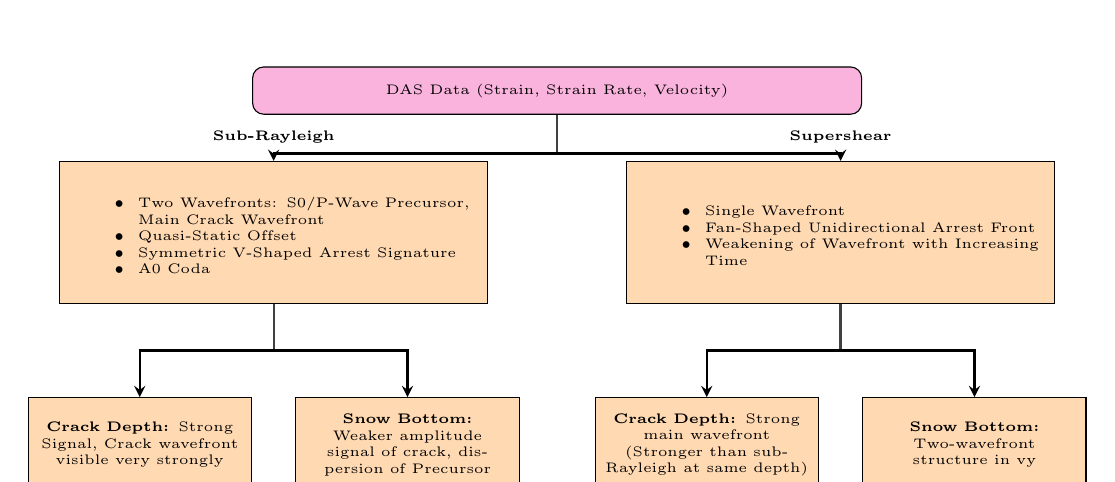
\begin{tikzpicture}

  
% ===============================
    % 1. NODES (Scaled for Portrait A4 \textwidth)
    % ===============================

    % Root Node
    \node[startstop, text width=7.5cm, minimum height=0.6cm] (root) at (0, 0) {
        DAS Data (Strain, Strain Rate, Velocity)
    };

    % -------------------------------
    % MAIN BRANCHES
    % -------------------------------
    % Left Branch (Sub-Rayleigh)
    \node[process, text width=5.2cm, minimum height=1.8cm, align=left] (leftbox) at (-3.6, -1.8) {
        \begin{itemize}
          \item Two Wavefronts: S0/P-Wave Precursor, Main Crack Wavefront
          \item Quasi-Static Offset
          \item Symmetric V-Shaped Arrest Signature
          \item A0 Coda 
        \end{itemize}
    };
    \node[font=\tiny\bfseries, above=0.1cm of leftbox] (leftlabel) {
        Sub-Rayleigh
    };

    % Right Branch (Supershear)
    \node[process, text width=5.2cm, minimum height=1.8cm, align=left] (rightbox) at (3.6, -1.8) {
        \begin{itemize}
          \item Single Wavefront
          \item Fan-Shaped Unidirectional Arrest Front
          \item Weakening of Wavefront with Increasing Time
        \end{itemize}
    };
    \node[font=\tiny\bfseries, above=0.1cm of rightbox] (rightlabel) {
       Supershear
    };

    % -------------------------------
    % LEAF NODES (Bottom)
    % -------------------------------
    % Left-Left Leaf
    \node[process, text width=2.6cm, minimum height=1.2cm] (left_leaf_1) at (-5.3, -4.5) {
        \textbf{Crack Depth:} Strong Signal,  Crack wavefront visible very strongly
    };
    
    % Left-Right Leaf
    \node[process, text width=2.6cm, minimum height=1.2cm] (left_leaf_2) at (-1.9, -4.5) {
        \textbf{Snow Bottom:} Weaker amplitude signal of crack, dispersion of Precursor
    };

    % Right-Left Leaf
    \node[process, text width=2.6cm, minimum height=1.2cm] (right_leaf_1) at (1.9, -4.5) {
        \textbf{Crack Depth:} Strong main wavefront (Stronger than sub-Rayleigh at same depth)
    };
    
    % Right-Right Leaf
    \node[process, text width=2.6cm, minimum height=1.2cm] (right_leaf_2) at (5.3, -4.5) {
        \textbf{Snow Bottom:} Two-wavefront structure in vy
    };


    % ===============================
    % 2. CONNECTIONS
    % ===============================

    % Root to Main Boxes
    \draw[thick, draw=idea-dark] (root.south) -- (0, -0.8);
    \draw[arrow] (0, -0.8) -| (leftbox.north);
    \draw[arrow] (0, -0.8) -| (rightbox.north);

    % Left Box to Left Leaves
    \draw[thick, draw=idea-dark] (leftbox.south) -- (-3.6, -3.3);
    \draw[arrow] (-3.6, -3.3) -| (left_leaf_1.north);
    \draw[arrow] (-3.6, -3.3) -| (left_leaf_2.north);

    % Right Box to Right Leaves
    \draw[thick, draw=idea-dark] (rightbox.south) -- (3.6, -3.3);
    \draw[arrow] (3.6, -3.3) -| (right_leaf_1.north);
    \draw[arrow] (3.6, -3.3) -| (right_leaf_2.north);

\end{tikzpicture}
\caption{Graphical Representation to Identify Different Signatures in DAS}
\label{fig:das_identification}
\end{figure}



% \section{Comparison between pure SE and MPM}

% \subsection{Propagation speeds \& wavefronts observed}
% two wavefront strcuture might not be observed because speeds are much closer (propagation and p-wave speed)

% \subsection{Precursor \& Rupture Signature}

% In the sub-Rayleigh case in section \ref{sec:simple_disc}, a precursor was identified, which travels in positive direction of propagation at the S0 wave speed in all plots. In some of the sub-Rayleigh plots in the simple case, for example strain and strain rate at the snow bottom in figure \ref{fig:sub_strain}, this wavefront can also be observed propagating in the negative direction. In the MPM-guided simulations, a wavefront with speeds close to S0 and the p-wave speed was observed propagating in the positive as well as the negative direction of propagation in all plots.\textcolor{magenta}{explain why} \par

% While this precursor is weak in amplitude in the simple case plots, it can be seen clearly in the MPM-guided results. \textcolor{magenta}{why?}. This comparison is important for the interpretation of DAS field data, because the precursor might not always look the same. The different amplitudes but also polarity structure of the precursor S0 wave leads to the conclusion that it can be best identified via its speed. \par

% \subsection{Quasi-Static Wavefield}

% In the MPM-guided simulations, discussed in section \ref{sec:mpm_disc}, the quasi-static displacement field can be observed clearly as broad red and blue wavefronts. Such structures cannot be observed in the sub-Rayleigh simple case nor the Supershear simple case. The reason for this is the source wavelet used. While the ricker wavelet, which was used in the simple case, is symmetric \parencite{kAkiRichards19801981}, the MPM STFS are not symmetric. This means that their cumulative integral, unlike that of the ricker, is nonzero \parencite{kaganPointSourcesElastic1987, zhuNoteDynamicStatic2002,freundDynamicFractureMechanics1998}, which leads to a net deformation, which is negative in this case. \par 

% \subsection{Wave types observed}

% \subsection{Crack arrest signatures}
% crack arrest much broader in mpm case






% \begin{itemize}
%   \item Compare fk plots and slopes measured: which propagation regime is observed in mpm?
%   \item Quasi-static offset comparison: why absent in simple model and why in MPM, what implications does this have
%   \item COmparison between wavefront structures: eg precursor
%   \item Comparison between types of waves present: which Lambwave modes and why
%   \item Crack arrest signature comparisons
%   \item Why absence / presence of dispersion and spreading? 
% \end{itemize}

%
% tex/sections/outlook.tex
% ──────────────────────────────────────────────────────────────────────────────
\chapter{Outlook}
\label{chap:outlook}
% ──────────────────────────────────────────────────────────────────────────────
%
% TODO: Write outlook.
%
% Suggested structure:
%   - Future work directly motivated by this thesis
%   - Broader research directions opened up
%   - Proposed experiments or improvements to methodology

Based on the results and methods presented in this thesis, there are many open lines of inquiry. Because the model described is a basic two layer model, a next step could be to add multiple layers, especially because cracks in snow usually propagate in a weak layer \parencite{schweizerSnowAvalancheFormation2003}. \par

There is also the possibility of adding topography or a slope angle to the simulation, because as indicated by \cite{anceySnowAvalanches2001,trottetTransitionSubRayleighAnticrack2022}, avalanches are gravity driven and the crack propagation regimes can change greatly with the presence of topography. \par 

There is the possibility for transition between the different propagation regimes, meaning that the propagation speed changes, as described by \cite{trottetTransitionSubRayleighAnticrack2022}, which is not only driven by topography and slope angle. Another next step would be to have source propagation accelerate with increasing propagation distance, instead of having a constant propagation speed, which is not very plausible on a mountain slope. \par 

%
% tex/sections/conclusion.tex
% ──────────────────────────────────────────────────────────────────────────────
\chapter{Conclusion}
\label{chap:conclusion}
% ──────────────────────────────────────────────────────────────────────────────
%
% TODO: Write conclusion.
%
% Suggested structure:
%   - Restate the objectives
%   - Summarise key findings (no new content)
%   - Broader significance / take-home message

% Opening: restate research objective in one sentence
% (~2 sentences)

The aim of this thesis was to contribute to the understanding of seismic signatures of crack propagation and avalanche breakoff. This was done
by setting up a moving-source model of a crack propagating at sub-rayleigh and supershear speeds in snow using spectral element modelling in SALVUS. The results of the simple two-layer model were evaluated to determine how the seismic signature measured by a DAS cable is influenced by the crack propagation regime. To make the physics more realisitic, the cohesive zone model for mixed-mode crack propagation was set up. This was then followed by a model which translated the results of material point method simulations by \cite{trottetTransitionSubRayleighAnticrack2022} into seismic moment tensors. The results of this simulation were evaluated to verify effects observed in the simple model at more realistic conditions. 

\section*{Answer to research questions}

% RQ1: FE modelling framework
% One paragraph: SALVUS spectral element method, two-layer and
% five-layer geometry, custom STF from MPM, DAS via pyber gauge length.
% One sentence on key assumptions (elastic, homogeneous, 2D, prescribed speed).

% RQ2: Physical phenomena in simple model
% One paragraph per main finding:
%   - Two-wavefront structure in sub-Rayleigh (S0 precursor + crack front)
%   - Single merged front in supershear (vr ≈ vp)
%   - A0 Lamb mode dominance (polarity reversal evidence)
%   - Arrest signatures (fan vs V-shape)
%   - Amplitude difference (10× more energy in supershear)

% RQ3: MPM-guided results
% One paragraph:
%   - Sub-Rayleigh confirmed at realistic parameters (vr ≈ 57 m/s)
%   - Quasi-static strain field (DC component, absent from simple model)
%   - Five-layer geometry validates simple model signatures

% RQ4: Implications for DAS detection
% One paragraph (your most important result):
%   - Sub-Rayleigh may be undetectable at snow bottom
%   - Arrest signature distinguishes regimes
%   - False conclusion risk if only supershear phase detected
%   - Quasi-static field as potential early warning

\section*{Limitations}

% Bullet or short paragraph covering:
%   - 2D geometry (no along-slope propagation, no azimuth variation)
%   - Elastic only (no attenuation, no viscous effects)
%   - Prescribed rupture speed (not self-consistent)
%   - Homogeneous layers (no spatial variability in weak layer)
%   - No field validation of simulated DAS signatures

\section*{Recommendations for future work}

% Point to outlook chapter or summarise in 3-4 sentences:
%   - 3D extension for arbitrary cable orientation
%   - Self-consistent rupture speed from cohesive zone model
%   - Field data comparison (PST with DAS)
%   - Heterogeneous weak layer properties



The subfault onset time is given by $\boldsymbol{t_o}$.
\nomenclature{$\boldsymbol{t_o}$}{Subfault onset time [s], e.g. $t_o=(x-x_{\rm start})/v_{\rm rupture}$.}

Horizontal coordinates match $\boldsymbol{x}$.
\nomenclature{$\boldsymbol{x},\,\boldsymbol{x}_{\rm start}$}{Horizontal coordinate and rupture starting position [m].}
%
%% ── BACK MATTER ─────────────────────────────────────────────────────────────
\backmatter
%
% Appendix
% tex/appendix.tex
% ──────────────────────────────────────────────────────────────────────────────
\begin{appendices}
%
\chapter{Appendix Title}
\label{app:A}

% TODO: Add appendix content — additional figures, derivations, tables, etc.

Lorem ipsum dolor sit amet, consectetur adipiscing elit. Replace this
placeholder with your appendix content.

\end{appendices}

%
% Bibliography
\cleardoublepage
\printbibliography[heading=bibintoc, title={Bibliography}]
%
\end{document}
